\documentclass{ctexart}

\usepackage{appendix}
\usepackage{listings}% 插入代码
\usepackage{xcolor} 
\usepackage{graphicx}% 插入表格/图片
\usepackage{booktabs} % 绘制表格
\usepackage{caption} % 标题
\usepackage{geometry}
\usepackage{array}
\usepackage{amsmath}
\usepackage{subfigure} % 插入图片
\usepackage{longtable}
\usepackage{abstract}% 摘要
\pagestyle{plain} % 页眉消失
\usepackage{setspace}
\usepackage{multirow}% 表格
\usepackage{diagbox}
\usepackage{enumerate}% 序号
\usepackage{float}% 固定图片或表格的位置
\usepackage{gensymb}
\usepackage{microtype}
\usepackage{hyperref}% 导航窗格

\geometry{a4paper,left=2.5cm,right=2.5cm,top=2cm,bottom=2cm}% 页边距
\lstset{
    numbers=left, % 设置行号位置
    numberstyle=\tiny, % 设置行号大小
    keywordstyle=\color{blue}, % 设置关键字颜色
    commentstyle=\color[cmyk]{1,0,1,0}, % 设置注释颜色
    escapeinside=``, % 逃逸字符(1左面的键),用于显示中文
    breaklines, % 自动折行
    extendedchars=false, % 解决代码跨页时,章节标题,页眉等汉字不显示的问题
    xleftmargin=1em,xrightmargin=1em, aboveskip=1em, % 设置边距
    tabsize=4, % 设置tab空格数
    showspaces=false % 不显示空格
}

\title{嫦娥三号软着陆轨道设计与控制策略}
\date{}
\author{}

\begin{document}
\maketitle
\renewcommand{\abstractname}{\Large\textbf{摘要}\\} % 使用 \huge 调整字体大小
\vspace{-4em} % 调整标题上间距
\begin{abstract}
\normalsize
本文针对嫦娥三号软着陆轨道设计与控制策略问题,建立了嫦娥三号的动力学微分方程和差分方程,着陆点选择模型与误差分析模型,解决了最优着陆轨道选取及控制问题。

针对问题一,提取关于月球与嫦娥三号的参数,根据所给椭圆轨道和月球位置,利用万有引力定律,计算出嫦娥三号在轨道近月点和远月点的轨道速度和方向。之后再建立嫦娥三号在主减速阶段的动力学方程,将油耗最小作为优化目标,结合始末状态的参数作为约束条件,离散求解\textbf{微分方程},即得降落轨道的数值解:\textbf{近月点速度$v_p = 1692.20 \, \text{m/s}$,远月点速度
$v_a = 1613.90 \, \text{m/s}$,近月点经纬度为(19.41°W,31.48°N),远月点经纬度为(160.59°E,31.48°S)。}

针对问题二,根据题意可分为六个阶段,首先对主减速阶段和快速调整阶段建立物理模型,以油耗最小作为优化目标,结合每一阶段始末状态的参数作为约束条件,离散求解动力学微分方程,对推力方向和速度方向进行搜索,得出最优推力方向的夹角,求解油耗最低的着陆策略,前两阶段\textbf{最终油耗为1104.563\(kg\)。}
其次在粗避障阶段,先选取着陆点,首先对高程图进行\textbf{高斯滤波}平滑处理,接下来进行梯度计算,将数据分块计算平均梯度,降低计算复杂度,能够分析局部区域的特性,并反转其灰度值,综合考虑地区平坦程度与油耗大小,创建\textbf{径向衰减掩码}并应用到反转的梯度图上,最后对掩码后的平均梯度进行排序,得出\textbf{最佳着陆点为(1122.5 1142.5)。}在精避障阶段,将始末状态的参数作为约束条件,离散求解动力学微分方程,\textbf{当前阶段末速度:15.274\(m/s\),精避障阶段末质量:1251.483\(kg\),当前燃油消耗质量:1148.517\(kg\),当前阶段末高度:30.092\(m\),最终在经过缓速下降与自由落体阶段,总着陆时间:533.179\(s\),自由落体阶段末质量:1242.592\(kg\),总燃油消耗质量:1157.405\(kg\)。}

针对问题三,将误差分为两个部分:\textbf{物理误差与控制误差}。综合考虑地球重力场与基于行星历表的其他星体引力场,太阳光压与大气模型,质量瘤影响,固体潮效应和相对论效应等物理误差,分别计算可能的误差情况并计算哪些误差影响,重要性排序为质量瘤引力变化,太阳引力,地球引力,木星引力,大气阻力,相对论效应引力,固体潮引力。并综合考虑求解精度影响和发动机推力控制误差与着陆准备轨道的参数误差等控制误差,得出初始值对于最终结果的影响。利用\textbf{四阶龙格-库塔法},得知求解进度对误差的影响较小,最终进行对于初始值的敏感性分析,并利用\textbf{蒙特卡罗方法}得出仿真结果,发现降落点集中在一定区域内,得出敏感性较好。

\textbf{关键词}:动力学\  \ 微分方程\  \ 差分方程\  \ 径向衰减掩码\  \ 蒙特卡罗方法
\end{abstract}
\newpage

% 重新设置页面边距
    \newgeometry{a4paper,left=3.18cm,right=3.18cm,top=2.54cm,bottom=2.54cm}
	\section{问题背景与重述}
	\subsection{问题背景}
    嫦娥三号于2013年12月2日1时30分成功发射,12月6日抵达月球轨道。嫦娥三号在着陆准备轨道上的运行质量为2.4t,其安装在下部的主减速发动机能够产生1500N到7500N的可调节推力,其比冲(即单位质量的推进剂产生的推力)为2940m/s,可以满足调整速度的控制要求。在四周安装有姿态调整发动机,在给定主减速发动机的推力方向后,能够自动通过多个发动机的脉冲组合实现各种姿态的调整控制。嫦娥三号的预定着陆点为19.51W,44.12N,海拔为-2641m(见附件1)。

嫦娥三号在高速飞行的情况下,要保证准确地在月球预定区域内实现软着陆,关键问题是着陆轨道与控制策略的设计。其着陆轨道设计的基本要求:着陆准备轨道为近月点15km,远月点100km的椭圆形轨道;着陆轨道为从近月点至着陆点,其软着陆过程共分为6个阶段(见附件2),要求满足每个阶段在关键点所处的状态;尽量减少软着陆过程的燃料消耗。
    \subsection{问题表述}
    \begin{enumerate}[(1)]
        \item 问题一:确定着陆准备轨道近月点和远月点的位置,以及嫦娥三号相应速度的大小与方向。
        \item 问题二:确定嫦娥三号的着陆轨道和在6个阶段的最优控制策略。
        \item 问题三:对于你们设计的着陆轨道和控制策略做相应的误差分析和敏感性分析。
    \end{enumerate}

    \section{问题分析}
    \subsection{问题一分析}
    对于问题一,根据题干,提取出关于月球与嫦娥三号的参数,再根据所给椭圆形轨道和月球位置,利用万有引力定律,计算出嫦娥三号在轨道近月点和远月点的轨道速度和方向。之后再建立嫦娥三号在主减速阶段的动力学方程,将油耗最小作为优化目标,主减速阶段的动力学方程,油耗公式再结合始末状态的参数,离散求解微分方程,即得降落轨道的数值解。

    \subsection{问题二分析}
    在主减速阶段,基于问题一所给的动力学方程,以及完成了主减速阶段的计算,接下来对快速调整阶段与粗避障阶段分别建立物理模型并进行优化,加入着陆点选择模型,综合考虑平整度与油耗,基于此对精避障阶段进行分析与优化,最终对缓慢下降与自由落体阶段完成建模。

对于图形预处理方法,选用了高斯滤波,通过这种组合方法,选点既考虑了地形的平缓程度,也考虑了与中心的距离,即油耗。这种方法确保选点在实际应用中的有效性。
    \subsection{问题三分析}
    对于该问题,从控制策略与物理误差进行误差分析,并考虑
微分方程离散化的误差。

综合考虑地球重力场与基于行星历表的其他星体引力场,太阳光压与大气模型,质量瘤影响,固体潮效应和相对论效应,分别计算可能的误差情况并计算哪些误差影响最大。并综合考虑求解精度影响和发动机推力控制误差与着陆准备轨道的参数误差。最终进行对于初始值的敏感性分析,并利用蒙特卡罗方法得出仿真结果。
    \section{模型假设}
    \begin{enumerate}[(1)]
        \item 降落过程中,轨道都满足是开普勒轨道,忽略摄动。
        \item 距离微小时,使用姿态调整发动机,不必使用主发动机。
        \item 使用月球平均半径。
        \item 不考虑月球自转。
    \end{enumerate}

    \section{符号说明}
\begin{center}
    \setlength{\tabcolsep}{9mm}{
        \begin{tabular}{ccc}
            \specialrule{1.2pt}{0pt}{0pt} % 设置顶部粗线
            \textbf{符号} & \textbf{意义} & \textbf{单位}\\
            \midrule  % 设置中间横线
            \textnormal{F} & \textnormal{引力} & \textnormal{N}\\

\textnormal{M} & \textnormal{月球质量} & \textnormal{kg}\\
            \textnormal{m} & \textnormal{嫦娥三号质量} & \textnormal{kg}\\
            \textnormal{alpha} & \textnormal{推力方向与速度方向夹角} & \textnormal{rad}\\
				\textnormal{G} & \textnormal{万有引力常数} & \textnormal{\( \text{N} \cdot \text{m}^2 / \text{kg}^2 \)} \\
\textnormal{$h_p$} & \textnormal{近月点距离} & \textnormal{15 \, \text{km}} \\
\textnormal{$h_a$} & \textnormal{远月点距离} & \textnormal{100 \, \text{km}} \\
            \specialrule{1.2pt}{0pt}{0pt} % 设置底部粗线
        \end{tabular}
    }
\end{center}

    \section{模型建立与求解}
    \subsection{问题一模型的建立与求解}

    \subsubsection{问题一模型的建立}
对于问题一,根据题干,提取出关于月球与嫦娥三号的参数,再根据所给椭圆形轨道和月球位置,利用万有引力定律,计算出嫦娥三号在轨道近月点和远月点的轨道速度和方向。之后再建立嫦娥三号在主减速阶段的动力学方程,将油耗最小作为优化目标,主减速阶段的动力学方程,油耗公式再结合始末状态的参数,离散求解微分方程,即得降落轨道的数值解。

    \subsubsection{笛卡尔坐标系的建立}
以月球中心为原点,构建一个三维笛卡尔坐标系,其三个坐标轴分别为:

\begin{enumerate}
    \item \(X\) 轴:指向月球赤道平面与月球自转轴的交点方向,该方向与地球中心连线的方向重合。
    \item \(Y\) 轴:垂直于 \(X\) 轴,并且位于月球赤道平面内,与 \(X\) 轴构成一个直角平面。
    \item \(Z\) 轴:沿着月球自转轴指向北极。
\end{enumerate}

在该坐标系下,月球表面任意一点的位置可以用 \((X, Y, Z)\) 三个坐标值表示,这些值可以通过月面测量数据或卫星观测数据确定。这个坐标系不仅有助于定位月球表面特征(如陨石坑、山脉等),还可以用于分析月球探测器的轨道和运动状态。

为了进一步明确各个坐标轴的定义和使用场景,我们可以参考以下具体步骤:

\begin{enumerate}
    \item \textbf{确定 \(X\) 轴方向}:选择通过月球中心并指向地球中心的直线作为 \(X\) 轴。这一方向是由于月球总是以同一面朝向地球的特性决定的,因此是一个自然且稳定的参考方向。
    \item \textbf{定义 \(Z\) 轴}:沿月球自转轴指向月球北极。月球自转轴的方向可以通过天文观测确定,并且相对地球来说也是稳定的。
    \item \textbf{确定 \(Y\) 轴}:\(Y\) 轴垂直于 \(X\) 轴和 \(Z\) 轴,并与它们构成一个右手坐标系。具体来说,若使用右手法则,拇指指向 \(X\) 轴,食指指向 \(Y\) 轴,中指指向 \(Z\) 轴。
\end{enumerate}

通过建立上述笛卡尔坐标系,我们可以系统地进行月球探测数据的收集、分析和比较,为科学研究和月球探测任务提供一个标准化的参考框架。为简化问题,将其转换为二维坐标系。
    \subsubsection{轨道动力学模型的建立}

% 开普勒定律和万有引力方程
% 万有引力定律

由万有引力定律得:
\begin{equation}
F_{\text{引}} = G \frac{M_1 M_2}{r^2}
\label{eq:gravity}
\end{equation}

其中,\( F_{\text{引}}\) 表示两个质量分别为 \( M_1 \) 和 \( M_2 \) 的物体之间的引力,两个物体间距离为 \( r \)。\( G \) 是引力常数,其值约为 

\[
G = 6.67 \times 10^{-11} \, \text{N} \cdot \text{m}^2 / \text{kg}^2
\].

% 天体运动和开普勒定律

因为向心力由万有引力所提供,由牛顿第二定律得
\begin{equation}
F_{\text{引}} = m \frac{v^2}{r}
\label{eq:centripetal}
\end{equation}

此公式描述了天体在轨道上的向心力(也即轨道动力学),其中 \( m \) 是天体的质量,\( v \) 是轨道速度,\( r \) 是轨道半径。

% 综合模型
由公式 (\ref{eq:gravity}) 与 (\ref{eq:centripetal}) 得:
\begin{equation}
G \frac{M_1 M_2}{r^2} = m \frac{v^2}{r}
\label{eq:3}
\end{equation}

展示了引力在天体轨道运动中的作用,即引力提供了向心力,使得天体能够沿着轨道运动。这一模型常用于天体物理学和轨道力学中,来分析行星、卫星等天体的轨道运动情况。

已知月球质量为

\[M = 7.3477 \times 10^{22} \, \text{kg}\]


月球平均半径为

\[r = 1737.015 \, \text{km}\]


根据题干内容可知近月点距离为

\[h_p = 15 \, \text{km}\]

远月点距离为

\[h_a = 100 \, \text{km}\]

由此可知,近月点到月球中心的距离为

\[\rho_p = r + h_p = 1752.015 \, \text{km}\]

远月点到月球中心的距离为

\[\rho_a = r + h_a = 1837.015 \, \text{km}\]

椭圆轨道半长轴长度为

\[a = \frac{\rho_p + \rho_a}{2} = 1794.515 \, \text{km}\]

% 计算c

椭圆轨道的焦距,即月球中心到椭圆轨道中心的距离为

\[c = a - \rho_p = 42.5 \, \text{km}\]

近月点和远月点处椭圆轨道的曲率为

\[\rho = \frac{b^2}{a} = \frac{a^2 - c^2}{a} = 1793.506 \, \text{km}\]

此刻,可由公式 (\ref{eq:3})变形为

\[G \frac{M m}{\rho_p^2} = m \frac{v_p^2}{\rho}\]
\[G \frac{M m}{\rho_a^2} = m \frac{v_a^2}{\rho}\]

将上述公式代入参数求解得

\[v_p = 1692.20 \, \text{m} / \text{s}\]
\[v_a = 1613.90 \, \text{m} / \text{s}\]

其中,\(v_p\)为嫦娥三号在着陆准备轨道近月点的速度,\(v_a\)为嫦娥三号在着陆准备轨道远月点的速度。

    \subsubsection{主减速阶段的动力学模型}
% 运动方程和燃料消耗方程
为解决嫦娥三号在着陆准备轨道的定位问题,需要从主减速末期倒推得出主减速阶段的起点,即着陆准备轨道的近月点。

在已建立的笛卡尔坐标系中,由牛顿第二定律\(F=ma\)
可得嫦娥三号在\(x\)轴方向的动力学微分方程为

\begin{equation}
\frac{M \sin(\theta)}{x^2 + y^2} + \frac{F \cos(\alpha + \theta)}{m} = \frac{d^2 x}{dt^2}
\end{equation}

嫦娥三号在\(y\)轴方向的动力学微分方程为

\begin{equation}
\frac{M \cos(\theta)}{x^2 + y^2} + \frac{F \sin(\alpha + \theta)}{m} = \frac{d^2 y}{dt^2}
\end{equation}

其中\(m\)为嫦娥三号的质量关于\(t\)的函数,\(\theta\)为嫦娥三号所受引力方向与\(y\)轴的夹角,\(\alpha\)为嫦娥三号所受推力方向与速度方向的夹角,关系式为:

\[\theta = \arctan \left( \frac{v_{y}}{{k}{v_{x}}} \right)\]

其中,考虑到题目要求要尽可能符合目标函数,即油耗最小,一开始设推力方向与速度方向相反,但这会导致速度达到57\(m/s\)前就会抵达降落点,所以此处遍历\(k\),取\(k\)为3.74684。

嫦娥三号的速度在\(x\)轴上的投影:
\[v_x = \frac{dx}{dt}\]

嫦娥三号的速度在\(x\)轴上的投影:
\[v_y = \frac{dy}{dt}\]

根据附件信息得

\begin{equation}
F_{\text{thrust}} = v_e \dot{m}
\end{equation}

其中,由题干可知,比冲\(v_e\)=2940\(m/s\),\(F_{\text{thrust}}\)是嫦娥三号发动机的推力,\(\dot{m}\)是单位时间燃料消耗的公斤数。

由此可得嫦娥三号的质量微分方程为

\begin{equation}
\frac{dm}{dt} = -\frac{F}{v_e} \\
\end{equation}

其中\(m\)为嫦娥三号的质量关于\(t\)的函数。

运动方程和燃料消耗方程:

\begin{equation}
\begin{cases}
\displaystyle \frac{M \sin(\theta)}{x^2 + y^2} + \frac{F \cos(\alpha + \theta)}{m} = \frac{d^2 x}{dt^2} \\
\displaystyle \frac{M \cos(\theta)}{x^2 + y^2} + \frac{F \sin(\alpha + \theta)}{m} = \frac{d^2 y}{dt^2} \\
\displaystyle \theta = \arctan\left( \frac{v_y}{k v_x} \right) \\
\displaystyle \frac{dm}{dt} = -\frac{F}{v_e} \\
\displaystyle \frac{dx}{dt} = v_x \\
\displaystyle \frac{dy}{dt} = v_y
\end{cases}
\end{equation}

% 运动方程和燃料消耗方程的详细介绍
这些方程表示物体在推力和引力作用下的运动:第一个方程表示 $x$ 方向的加速度,其由引力和推力的 $x$ 分量决定,第二个方程表示 $y$ 方向的加速度,其由引力和推力的 $y$ 分量决定。第三个方程表示质量随时间的变化,即燃料消耗率。第四个和第五个方程表示速度与位置的关系。


% 初始状态
初始状态:
\begin{equation}
\begin{cases}
\theta(0) = 0 \\
x(0) = 0 \\
y(0) = 15000 \, \text{m} \\
m(0) = 2400 \, \text{kg} \\
v_t(0) = 1700 \, \text{m/s} \\
v_n(0) = 0 \, \text{m/s}
\end{cases}
\end{equation}

% 初始状态的详细介绍

$\theta(0)$ 表示初始时刻的角度,
$x(0)$ 表示初始时刻的位置,
$y(0)$ 表示初始时刻的位置,
$m(0)$ 表示初始时刻的质量,
$v_t(0)$ 表示初始时刻的切向速度,
$v_n(0)$ 表示初始时刻的法向速度。

% 末状态
末状态:
\begin{equation}
\begin{cases}
y(t_1) = 3000 \, \text{m} \\
\sqrt{v_t(t_1)^2 + v_n(t_1)^2} = 57 \, \text{m/s}
\end{cases}
\end{equation}

% 末状态的详细介绍
% 使用自定义的itemize环境来去掉黑点
\begin{itemize}
    \renewcommand\labelitemi{} % 去掉项目符号
    \item $y(t_1)$ 表示最终时刻的位置。
    \item $\sqrt{v_t(t_1)^2 + v_n(t_1)^2}$ 表示最终时刻的速度大小。
\end{itemize}

	\subsubsection{主减速阶段的优化}
只有计算出最优的主减速轨道,才能回溯出着陆准备轨道精确的近月点位置。
% 目标函数
目标函数:
\begin{equation}
m_{\text{燃}} = \int_0^{t_1} \frac{F}{v_e} \, dt
\end{equation}

% 目标函数的详细介绍
% 使用自定义的itemize环境来去掉黑点
\begin{itemize}
    \renewcommand\labelitemi{} % 去掉项目符号
    \item 这个公式表示燃料消耗的目标函数,其中:
    \item $m_{\text{燃}}$ 是总燃料消耗量。
    \item $F$ 是推力,取7500\(N\)。
    \item $v_e$ 是以米/秒为单位的比冲。
    \item 积分的上下限是从初始时间 $0$ 到最终时间 $t_1$。
\end{itemize}

嫦娥三号到月球中心的距离\(r\)关于飞行时间\(t\)的差分方程为

\[r_{t+1} = r_t + v_t \Delta t + \frac{1}{2} a_t (\Delta t)^2\]

飞行速度\(v\)关于飞行时间\(t\)的差分方程为
\[v_{t+1} = v_t + a_t \Delta t\]

嫦娥三号的质量\(m\)关于飞行时间\(t\)的差分方程为
\[m_{t+1} = m_t - \dot{m} \Delta t\]

嫦娥三号所受月球引力施加的加速度大小为
\[a_g = - G \frac{M}{r^2}\]

嫦娥三号所受发动机推力施加的加速度大小为
\[a_n = \frac{F}{m}\]

嫦娥三号运动的总加速度大小为
\[a_t = a_g + a_n\]

嫦娥三号的动力学差分方程为
\[
\begin{cases}
r_{t+1} = r_t + v_t \Delta t + \frac{1}{2} a_t (\Delta t)^2 \\
v_{t+1} = v_t + a_t \Delta t \\
m_{t+1} = m_t - \dot{m} \Delta t \\
a_g = - G \frac{M}{r^2} \\
a_n = \frac{F}{m} \\
a_t = a_g + a_n
\end{cases}
\]

	\subsubsection{着陆准备轨道的计算结果}
着陆准备轨道的参数如下:
\begin{center}
    \setlength{\tabcolsep}{9mm}{
        \begin{tabular}{cc}
            \specialrule{1.2pt}{0pt}{0pt} % 设置顶部粗线
            \textbf{参数} & \textbf{值} \\
            \midrule  % 设置中间横线
            主减速阶段飞行时间 & 414.915 \(s\) \\
            主减速阶段末速度 & 56.998 \(m/s\) \\
            飞船主减速阶段末质量 & 1341.543 \(kg\) \\
            主减速阶段燃油消耗质量 & 1058.457 \(kg\) \\
            飞船主减速阶段末高度 & 2997.319 \(m\) \\
            \specialrule{1.2pt}{0pt}{0pt} % 设置底部粗线
        \end{tabular}
    }
\end{center}

    \begin{figure}[H] % [H] 表示强制当前位置插入图片
        \centering % 使图片居中
        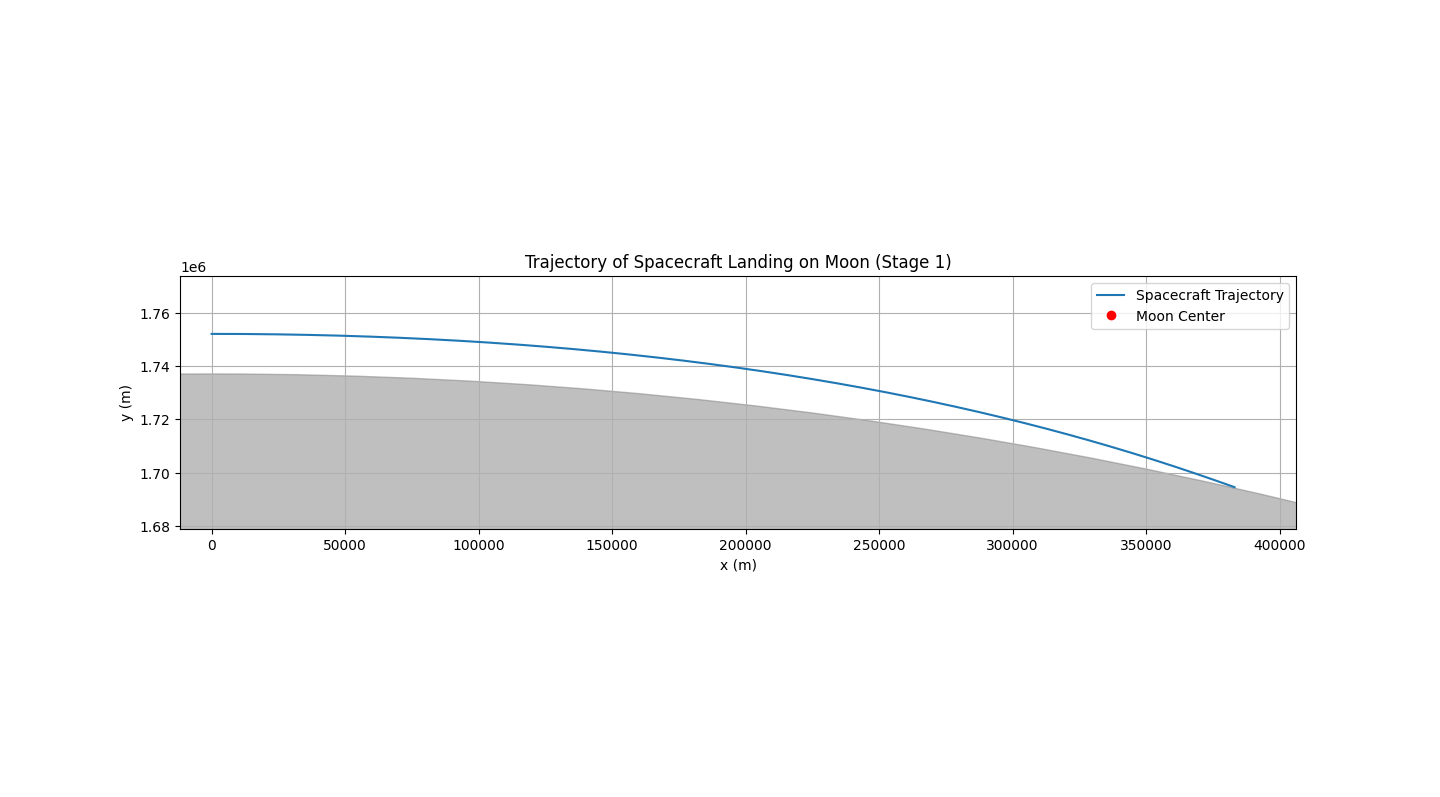
\includegraphics[width=0.8\textwidth]{"./picture/stage1.png"} % 图片文件名及宽度调整
        \caption{主减速阶段示意图} % 图片标题
        \label{fig:example} % 图片标签
    \end{figure}
	\subsubsection{问题的结论}

\[v_p = 1692.20 \, \text{m} / \text{s}\]
\[v_a = 1613.90 \, \text{m} / \text{s}\]

其中,\(v_p\)为嫦娥三号在着陆准备轨道近月点的速度,\(v_a\)为嫦娥三号在着陆准备轨道远月点的速度。
    \subsection{问题二模型的建立与求解}


\subsubsection{模型建立与求解}
优化设计六个阶段,分别对每个阶段建立物理模型,并利用优化,求解油耗最低的降落策略。

对于着陆点选取,首先进行梯度计算,将数据分块计算平均梯度并反转其灰度值,创建径向衰减掩码并应用于数据,最终对掩码后的平均梯度进行排序

对于着陆点的选取,对地面平整度与油耗进行赋权,得出最佳着陆点。

\subsubsection{着陆模型建立}
因为主减速阶段的轨道问题在问题一中已被解决,由此接下来可以继续对其他阶段继续分析。

分别对每个阶段建立物理模型,并利用优化,求解油耗最低的降落策略。又因为每一段的目标函数都是使得油耗最小,所以可得目标函数:
\begin{equation}
m_{\text{燃}} = \int_{t}^{T} \frac{F}{v_e} \, dt
\end{equation}

% 目标函数的详细介绍

其中:$m_{\text{燃}}$是总燃料消耗量,
$F$ 是推力,
$v_e$ 是以米/秒为单位的比冲,
积分的上下限是从初始时间 $t$ 到最终时间 $T$。


嫦娥三号到月球中心的距离\(r\)关于飞行时间\(t\)的差分方程为

\[r_{t+1} = r_t + v_t \Delta t + \frac{1}{2} a_t (\Delta t)^2\]

飞行速度\(v\)关于飞行时间\(t\)的差分方程为
\[v_{t+1} = v_t + a_t \Delta t\]

嫦娥三号的质量\(m\)关于飞行时间\(t\)的差分方程为
\[m_{t+1} = m_t - \dot{m} \Delta t\]

嫦娥三号所受月球引力施加的加速度大小为
\[a_g = - G \frac{M}{r^2}\]

嫦娥三号所受发动机推力施加的加速度大小为
\[a_n = \frac{F}{m}\]

嫦娥三号运动的总加速度大小为
\[a_t = a_g + a_n\]

嫦娥三号的动力学差分方程为
\[
\begin{cases}
r_{t+1} = r_t + v_t \Delta t + \frac{1}{2} a_t (\Delta t)^2 \\
v_{t+1} = v_t + a_t \Delta t \\
m_{t+1} = m_t - \dot{m} \Delta t \\
a_g = - G \frac{M}{r^2} \\
a_n = \frac{F}{m} \\
a_t = a_g + a_n
\end{cases}
\]

\subsubsection{快速调整阶段}
快速调整阶段的推力大小取3110.52\(N\)。

目标函数:
\begin{equation}
m_{\text{燃}} = \int_{t_1}^{t_2} \frac{F}{v_e} \, dt
\end{equation}

嫦娥三号的动力学差分方程为
\[
\begin{cases}
r_{t+1} = r_t + v_t \Delta t + \frac{1}{2} a_t (\Delta t)^2 \\
v_{t+1} = v_t + a_t \Delta t \\
m_{t+1} = m_t - \dot{m} \Delta t \\
a_g = - G \frac{M}{r^2} \\
a_n = \frac{F}{m} \\
a_t = a_g + a_n
\end{cases}
\]

初始状态:
\begin{equation}
\begin{cases}
y(t_1) = 2997.319 \, \text{m} \\
m(t_1) = 1341.543 \, \text{kg} \\
v_t(t_1) = 6.592 \, \text{m/s} \\
v_n(t_1) = 56.616 \, \text{m/s}
\end{cases}
\end{equation}

% 初始状态的详细介绍

$y(t_1)$ 表示初始时刻的位置,
$m(t_1)$ 表示初始时刻的质量,
$v_t(t_1)$ 表示初始时刻的切向速度,
$v_n(t_1)$ 表示初始时刻的法向速度。

% 末状态
末状态:
\begin{equation}
\begin{cases}
y(t_2) = 2400 \, \text{m} \\
{v_t(t_2)} = 0 \, \text{m/s}
\end{cases}
\end{equation}

% 末状态的详细介绍
\begin{itemize}
    \renewcommand\labelitemi{} % 去掉项目符号
\item $y(t_2)$ 表示最终时刻的位置。
\item ${v_t(t_2)}$ 表示最终时刻的速度水平速度大小。
\end{itemize}

    \begin{figure}[H] % [H] 表示强制当前位置插入图片
        \centering % 使图片居中
        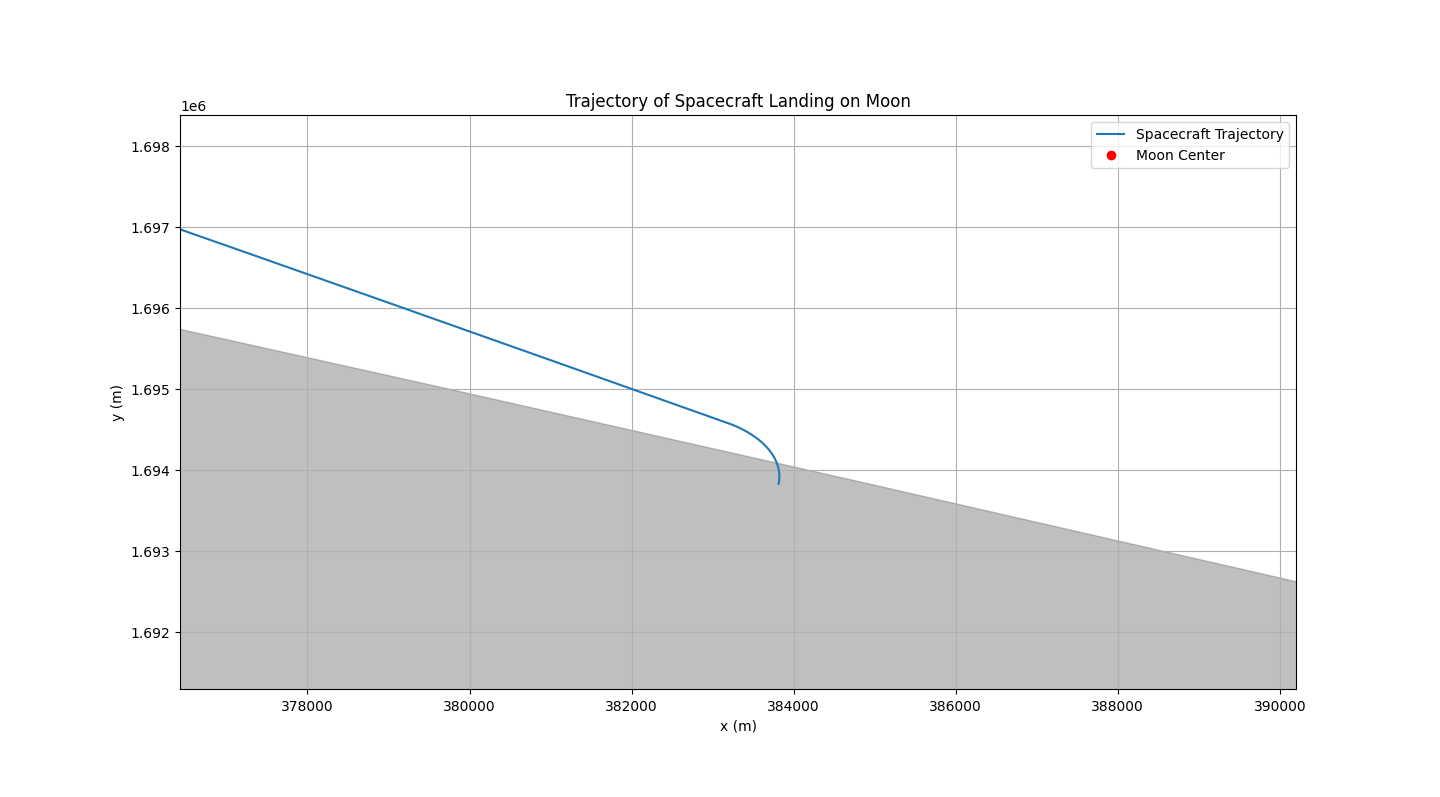
\includegraphics[width=0.6\textwidth]{"./picture/stage2.png"} % 图片文件名及宽度调整
        \caption{快速调整阶段示意图} % 图片标题
        \label{fig:example} % 图片标签
    \end{figure}
快速调整阶段参数如下:
\begin{center}
    \setlength{\tabcolsep}{9mm}{
        \begin{tabular}{cc}
            \specialrule{1.2pt}{0pt}{0pt} % 设置顶部粗线
            \textbf{参数} & \textbf{值} \\
            \midrule  % 设置中间横线
            总飞行时间 & 458.494 \(s\) \\
            当前阶段末速度 & 4.283 \(m/s\) \\
            当前阶段末水平速度 & 0.0999 \(m/s\) \\
            快速调整阶段末质量 & 1295.437 \(kg\) \\
            总燃油消耗质量 & 1104.563 \(kg\) \\
            当前阶段末高度 & 2397.449 \(m\) \\
            \specialrule{1.2pt}{0pt}{0pt} % 设置底部粗线
        \end{tabular}
    }
\end{center}

\subsubsection{图片预处理}
\textbf{高斯平滑}:

高斯平滑通过高斯滤波器对图像进行卷积,公式为:
\[
G(x, y) = \frac{1}{2\pi\sigma^2} \exp\left(-\frac{x^2 + y^2}{2\sigma^2}\right)
\]

在实际操作中,高斯平滑通常通过离散的高斯核进行卷积计算:
\[
I_{smooth}(x, y) = \sum_{i=-k}^{k} \sum_{j=-k}^{j} I(x-i, y-j) \cdot G(i, j)
\]
\subsubsection{降落点选择模型}

\textbf{梯度大小}:

梯度大小表示坡度的陡峭程度。较大的梯度表示坡度较陡,较小的梯度表示坡度较平缓。在反转梯度之后,较大的值表示较平缓的区域。定义梯度为:
\[
\nabla h = \left( \frac{\partial h}{\partial x}, \frac{\partial h}{\partial y} \right)
\]

其中,\( h \) 是高程值,\(\nabla h\) 是梯度向量。

梯度的大小(即坡度)可以表示为:
\[
|\nabla h| = \sqrt{\left( \frac{\partial h}{\partial x} \right)^2 + \left( \frac{\partial h}{\partial y} \right)^2}
\]

\textbf{径向衰减掩码}

径向衰减掩码的目的是对距离中心较远的区域施加更大的衰减。这样可以优先考虑中心区域的选点。径向衰减掩码可以表示为:

\[
\text{Mask}(x, y) = \frac{1}{k \cdot d(x, y) + 1}
\]

其中,\( k \) 是衰减速度常数,\( d(x, y) \) 是点 \((x, y)\) 到中心的距离,定义为:
\[
d(x, y) = \sqrt{(x - x_0)^2 + (y - y_0)^2}
\]

其中,\( (x_0, y_0) \) 是图像的中心坐标。

\textbf{组合应用}

反转后的平均梯度图与径向衰减掩码组合应用,得到最终的梯度图。在这个图中,梯度较小且距离中心较近的区域将得到更高的权重。组合应用可以表示为:

\[
\text{Final\_Gradient}(x, y) = (\max(\text{Gradient}) - \text{Gradient}(x, y)) \cdot \text{Mask}(x, y)
\]

其中,\(\text{Gradient}(x, y)\) 是点 \((x, y)\) 的梯度值,\(\max(\text{Gradient})\) 是梯度图中的最大值。

通过这种组合方法,选点既考虑了地形的平缓程度,也考虑了与中心的距离,即油耗。这种方法确保选点在实际应用中的有效性。
由此,我们所选点坐标为:[1122.5 1142.5],[1127.5 1147.5],[1142.5 1152.5],[1057.5 1157.5],[1127.5 1182.5]。

    \begin{figure}[H] % [H] 表示强制当前位置插入图片
        \centering % 使图片居中
        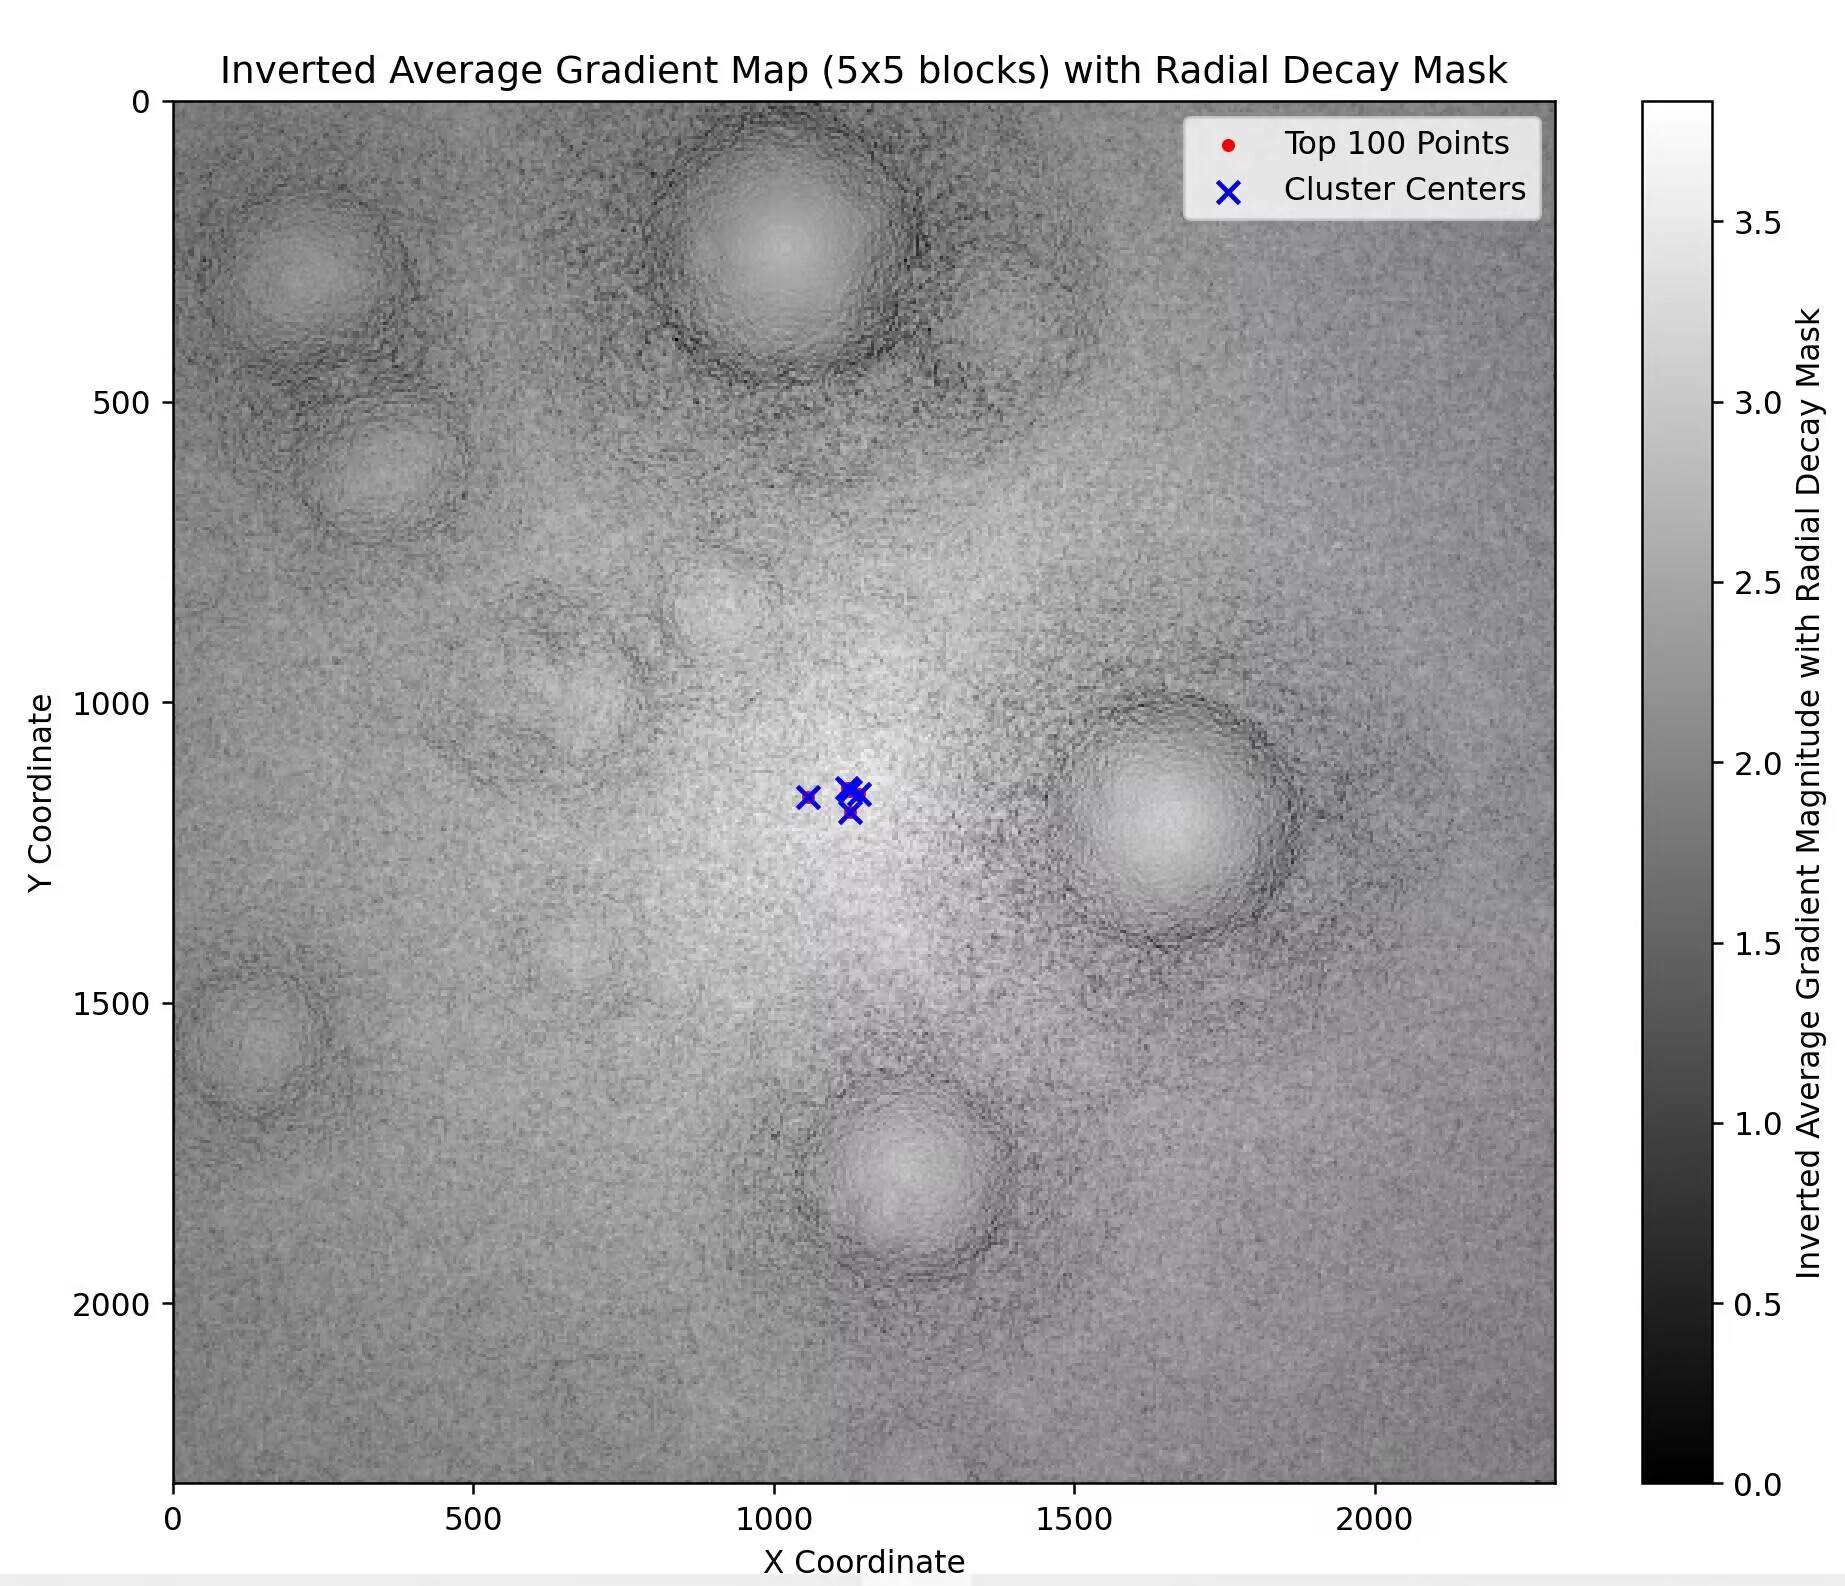
\includegraphics[width=0.6\textwidth]{"./picture/1.jpg"} % 图片文件名及宽度调整
        \caption{选点示意图} % 图片标题
        \label{fig:example} % 图片标签
    \end{figure}

\subsubsection{粗避障阶段}
先自由落体直至与降落点高度差为741\(m\),再以7500N推力反推,在距离目标上方100\(m\)处悬停。

目标函数:
\begin{equation}
m_{\text{燃}} = \int_{t_2}^{t_4} \frac{F}{v_e} \, dt
\end{equation}

嫦娥三号的动力学差分方程为
\[
\begin{cases}
r_{t+1} = r_t + v_t \Delta t + \frac{1}{2} a_t (\Delta t)^2 \\
v_{t+1} = v_t + a_t \Delta t \\
m_{t+1} = m_t - \dot{m} \Delta t \\
a_g = - G \frac{M}{r^2} \\
a_n = \frac{F}{m} \\
a_t = a_g + a_n
\end{cases}
\]

自由落体阶段末状态:
\begin{equation}
\begin{cases}
y(t_3) = 740.936 \, \text{m} \\
m(t_3) = 1295.437 \, \text{kg} \\
v_t(t_3) = 0.100 \, \text{m/s} \\
v_n(t_3) = 73.523 \, \text{m/s}
\end{cases}
\end{equation}

% 初始状态的详细介绍

$y(t_3)$ 表示中间时刻的位置,
$m(t_3)$ 表示中间时刻的质量,
$v_t(t_3)$ 表示中间时刻的切向速度,
$v_n(t_3)$ 表示中间时刻的法向速度。

% 末状态
末状态:
\begin{equation}
\begin{cases}
y(t_4) = 101.703 \, \text{m} \\
\sqrt{v_t(t_4)^2 + v_n(t_4)^2} = 0 \, \text{m/s}
\end{cases}
\end{equation}

% 末状态的详细介绍
\begin{itemize}
    \renewcommand\labelitemi{} % 去掉项目符号
\item $y(t_4)$ 表示最终时刻的位置。
\item $\sqrt{v_t(t_4)^2 + v_n(t_4)^2}$ 表示最终时刻的速度水平速度大小。
\end{itemize}

    \begin{figure}[H] % [H] 表示强制当前位置插入图片
        \centering % 使图片居中
        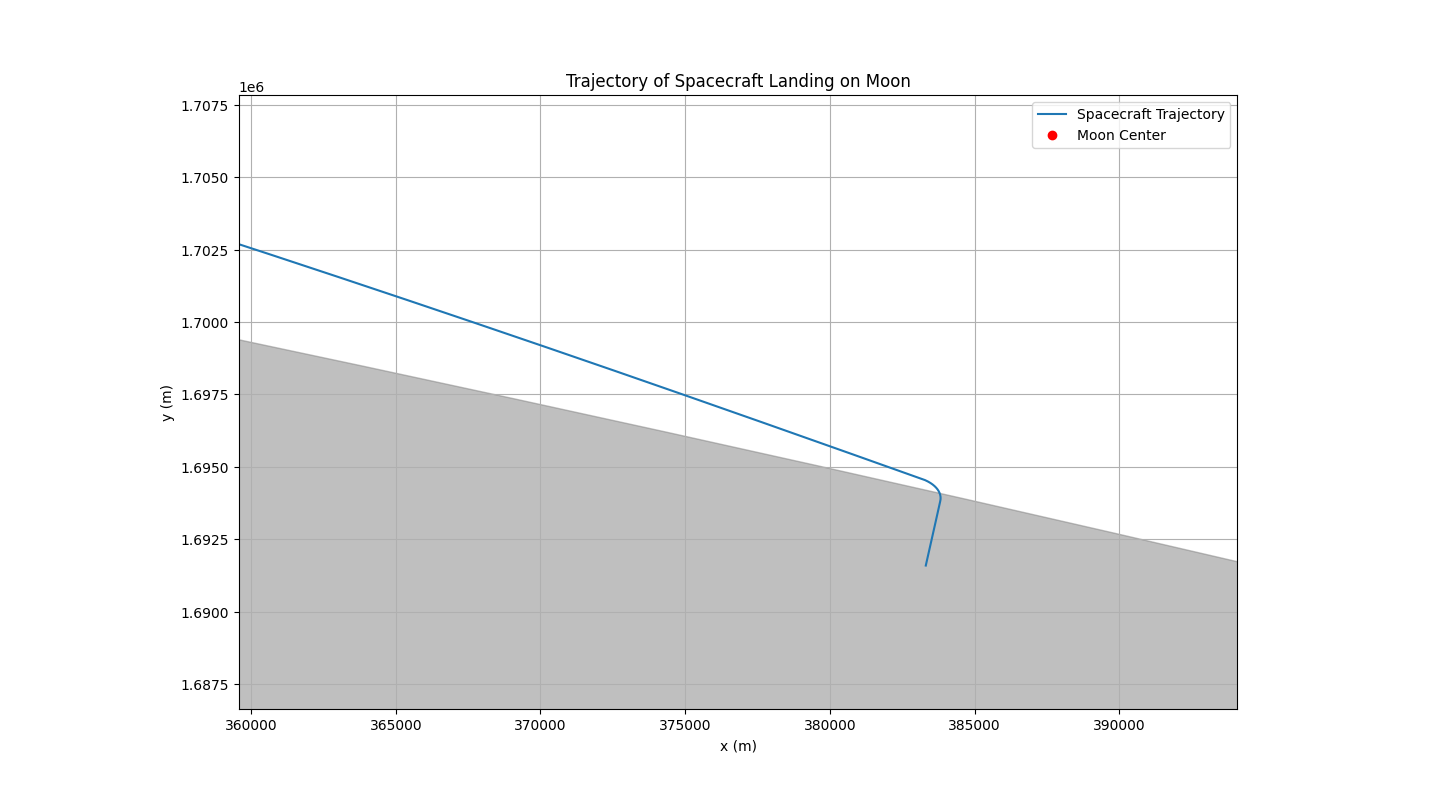
\includegraphics[width=0.7\textwidth]{"./picture/stage3_2.png"} % 图片文件名及宽度调整
        \caption{粗避障阶段示意图} % 图片标题
        \label{fig:example} % 图片标签
    \end{figure}
粗避障阶段参数如下:
\begin{center}
    \setlength{\tabcolsep}{9mm}{
        \begin{tabular}{cc}
            \specialrule{1.2pt}{0pt}{0pt} % 设置顶部粗线
            \textbf{参数} & \textbf{值} \\
            \midrule  % 设置中间横线
            总飞行时间 & 518.317 \(s\) \\
            当前阶段末速度 & 1.073 \(m/s\) \\
            粗避障阶段末质量 & 1251.483 \(kg\) \\
            总燃油消耗质量 & 1148.571 \(kg\) \\
            当前阶段末高度 & 101.703 \(m\) \\
            \specialrule{1.2pt}{0pt}{0pt} % 设置底部粗线
        \end{tabular}
    }
\end{center}
\subsubsection{精避障阶段}

目标函数:
\begin{equation}
m_{\text{燃}} = \int_{t_4}^{t_5} \frac{F}{v_e} \, dt
\end{equation}

嫦娥三号的动力学差分方程为
\[
\begin{cases}
r_{t+1} = r_t + v_t \Delta t + \frac{1}{2} a_t (\Delta t)^2 \\
v_{t+1} = v_t + a_t \Delta t \\
m_{t+1} = m_t - \dot{m} \Delta t \\
a_g = - G \frac{M}{r^2} \\
a_n = \frac{F}{m} \\
a_t = a_g + a_n
\end{cases}
\]

初始状态:

\begin{equation}
\begin{cases}
y(t_4) = 518.317 \, \text{m} \\
m(t_4) = 1251.483 \, \text{kg} \\
v_t(t_4) = 1.0683\times 10^{-5} \, \text{m/s} \\
v_n(t_4) = 0.0963 \, \text{m/s}
\end{cases}
\end{equation}

% 初始状态的详细介绍

$y(t_4)$ 表示初始时刻的位置,
$m(t_4)$ 表示初始时刻的质量,
$v_t(t_4)$ 表示初始时刻的切向速度,
$v_n(t_4)$ 表示初始时刻的法向速度。

% 末状态
末状态:
\begin{equation}
\begin{cases}
y(t_5) = 30 \, \text{m} \\
v_t(t_5) = 0 \, \text{m/s}
\end{cases}
\end{equation}

% 末状态的详细介绍
\begin{itemize}
\renewcommand\labelitemi{} % 去掉项目符号
\item $y(t_5)$ 表示最终时刻的位置。
\item $v_t(t_5)$ 表示最终时刻的速度水平速度大小。
\end{itemize}

    \begin{figure}[H] % [H] 表示强制当前位置插入图片
        \centering % 使图片居中
        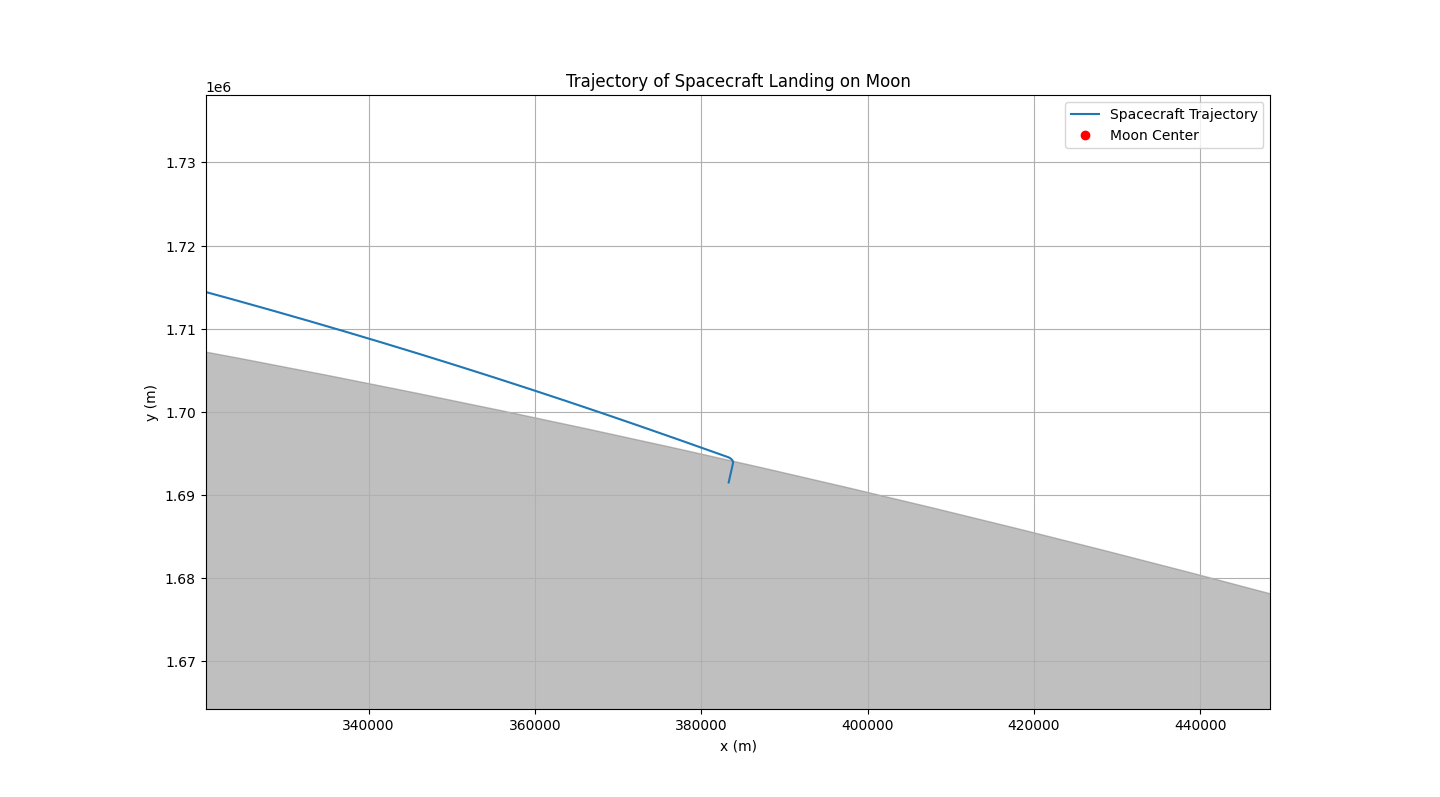
\includegraphics[width=0.7\textwidth]{"./picture/stage4.png"} % 图片文件名及宽度调整
        \caption{精避障阶段示意图} % 图片标题
        \label{fig:example} % 图片标签
    \end{figure}

精避障阶段参数如下:
\begin{center}
    \setlength{\tabcolsep}{9mm}{
        \begin{tabular}{cc}
            \specialrule{1.2pt}{0pt}{0pt} % 设置顶部粗线
            \textbf{参数} & \textbf{值} \\
            \midrule  % 设置中间横线
            总飞行时间 & 527.635 \(s\) \\
            当前阶段末速度 & 15.274 \(m/s\) \\
            粗避障阶段末质量 & 1251.483 \(kg\) \\
            总燃油消耗质量 & 1148.517 \(kg\) \\
            当前阶段末高度 & 30.092 \(m\) \\
            \specialrule{1.2pt}{0pt}{0pt} % 设置底部粗线
        \end{tabular}
    }
\end{center}
\subsubsection{缓慢下降与自由落体阶段}

目标函数:
\begin{equation}
m_{\text{燃}} = \int_{t_5}^{t_6} \frac{F}{v_e} \, dt
\end{equation}

嫦娥三号的动力学差分方程为
\[
\begin{cases}
r_{t+1} = r_t + v_t \Delta t + \frac{1}{2} a_t (\Delta t)^2 \\
v_{t+1} = v_t + a_t \Delta t \\
m_{t+1} = m_t - \dot{m} \Delta t \\
a_g = - G \frac{M}{r^2} \\
a_n = \frac{F}{m} \\
a_t = a_g + a_n
\end{cases}
\]

初始状态:
\begin{equation}
\begin{cases}
y(t_5) = 30.092 \, \text{m} \\
m(t_5) = 1251.483 \, \text{kg} \\
v_t(t_5) = 1.0683\times 10^{-5} \, \text{m/s} \\
v_n(t_5) = 15.274 \, \text{m/s}
\end{cases}
\end{equation}

% 初始状态的详细介绍

$y(t_3)$ 表示中间时刻的位置,
$m(t_3)$ 表示中间时刻的质量,
$v_t(t_3)$ 表示中间时刻的切向速度,
$v_n(t_3)$ 表示中间时刻的法向速度。

% 末状态
末状态:
\begin{equation}
\begin{cases}
y(t_6) = 3.447 \, \text{m} \\
\sqrt{v_t(t_6)^2 + v_n(t_6)^2} = 0 \, \text{m/s}
\end{cases}
\end{equation}

% 末状态的详细介绍
\begin{itemize}
\renewcommand\labelitemi{} % 去掉项目符号
\item $y(t_6)$ 表示最终时刻的位置。
\item $\sqrt{v_t(t_6)^2 + v_n(t_6)^2}$ 表示最终时刻的速度大小,因为此时悬停,因此速度为0。
\end{itemize}

    \begin{figure}[H] % [H] 表示强制当前位置插入图片
        \centering % 使图片居中
        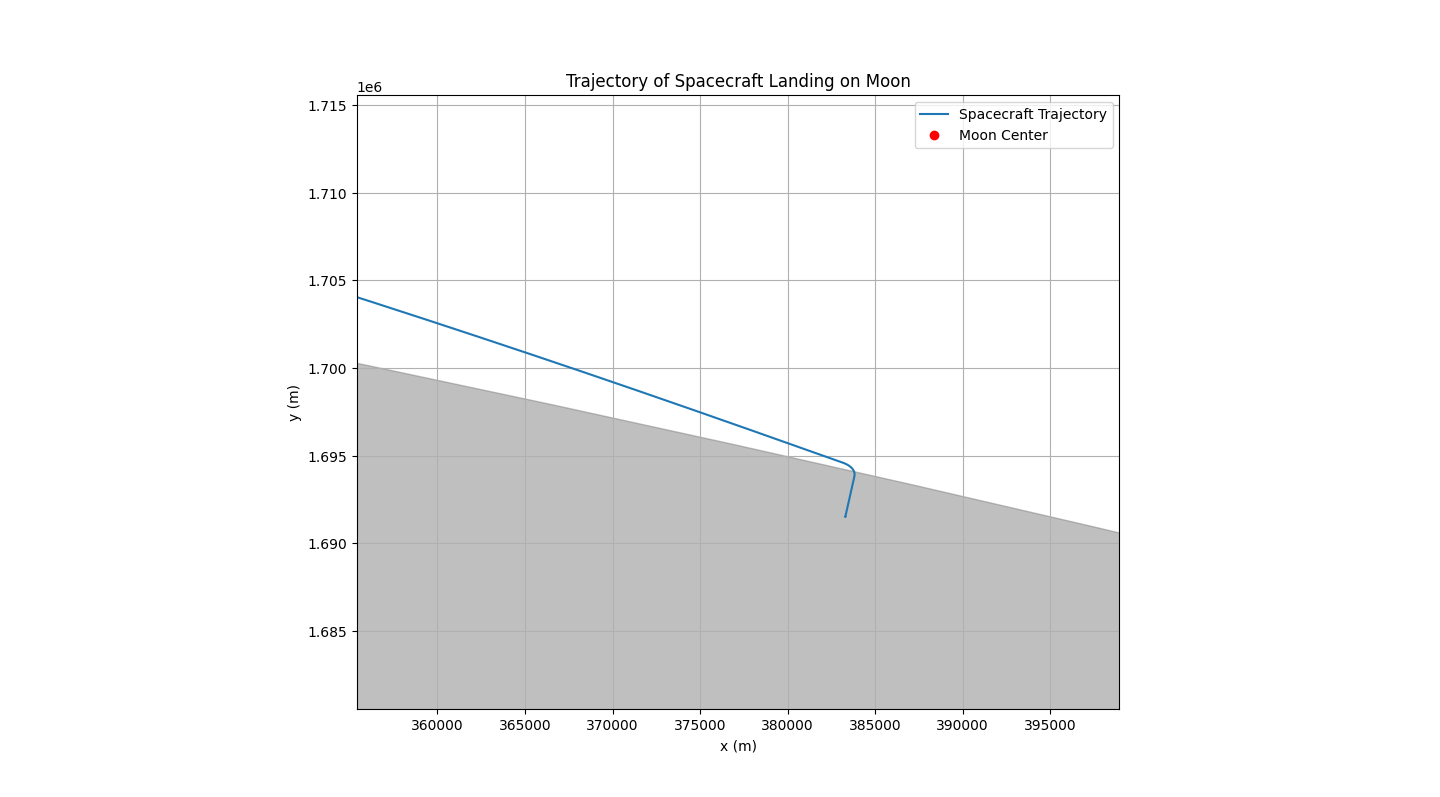
\includegraphics[width=0.8\textwidth]{"./picture/stage5.png"} % 图片文件名及宽度调整
        \caption{缓慢下降阶段示意图} % 图片标题
        \label{fig:example} % 图片标签
    \end{figure}

缓慢下降阶段参数如下:

\begin{center}
    \setlength{\tabcolsep}{9mm}{
        \begin{tabular}{cc}
            \specialrule{1.2pt}{0pt}{0pt} % 设置顶部粗线
            \textbf{参数} & \textbf{值} \\
            \midrule  % 设置中间横线
            总飞行时间 & 531.119 \(s\) \\
            当前阶段末速度 & $3.7 \times 10^{-3} \, \text{m/s}$ \\
            粗避障阶段末质量 & 1242.592 \(kg\) \\
            总燃油消耗质量 & 1157.405 \(kg\) \\
            当前阶段末高度 & 3.447 \(m\) \\
            \specialrule{1.2pt}{0pt}{0pt} % 设置底部粗线
        \end{tabular}
    }
\end{center}

由于缓慢下降阶段结束后,嫦娥三号悬停于目标上方并关闭了发动机,所以自由落体不消耗燃油。
自由落体运动结束后,状态参数为

\begin{center}
    \setlength{\tabcolsep}{9mm}{
        \begin{tabular}{cc}
            \specialrule{1.2pt}{0pt}{0pt} % 设置顶部粗线
            \textbf{参数} & \textbf{值} \\
            \midrule  % 设置中间横线
            总飞行时间 & 533.179 \(s\) \\
            自由落体阶段末质量 & 1242.592 \(kg\) \\
            总燃油消耗质量 & 1157.405 \(kg\) \\
            当前阶段末高度 & 0 \(m\) \\
            \specialrule{1.2pt}{0pt}{0pt} % 设置底部粗线
        \end{tabular}
    }
\end{center}
\subsubsection{问题的结论}
嫦娥三号的软着陆过程,总耗时533.179\(s\),总燃油消耗质量为1157.405\(kg\)。
    \subsection{问题三模型的建立与求解}
\subsubsection{模型求解}
分别是物理误差分析与控制误差。

控制论误差:求解精度影响和发动机推力控制误差与着陆准备轨道的参数误差

物理误差分析,摄动包括地球重力场,行星历表,太阳光压与相对论效益。

最终综合考虑地球重力场与基于行星历表的其他星体引力场,太阳光压与大气模型,质量瘤影响,固体潮效应和相对论效应,分别计算可能的误差情况并计算哪些误差影响最大。并综合考虑求解精度影响和发动机推力控制误差与着陆准备轨道的参数误差。最终进行对于初始值的敏感性分析,并利用蒙特卡罗方法得出仿真结果。
\subsubsection{误差分析导论}
进行误差分析对于登月飞行器轨道计算和控制具有重要意义,它能够提高精度,识别和量化各种误差来源,改进轨道计算和控制算法;进行风险评估和管理,制定应对策略,减少意外事件,提高任务可靠性;优化资源使用,集中资源优化关键部分,提升整体任务效率;制定校正策略,确保飞行器按预定轨道和姿态运行;提高系统鲁棒性,增强飞行器系统对各种扰动和不确定因素的适应能力;验证和改进设计,帮助工程师不断改进设计,提升系统性能。通过误差分析,可以确保登月飞行器任务的成功,并为未来类似任务提供宝贵的经验和数据。

误差分析:

1)模型的简化假设、模型的近似等物理误差的影响。



2)求解过程的精度误差影响。


3)分阶段分析发动机推力的控制误差的影响;

4)着陆准备轨道参数(位置和速度)的误差对实际着陆点的影响;
\subsubsection{地球重力场与基于行星历表的其他星体引力场}
在飞船着陆的过程中,其他星体的引力在一二问中并未考虑,而地球的引力对飞行器的影响最大。

根据牛顿万有引力定律,两物体之间的引力 \( F \) 由下式给出:
\[
F = \frac{G M_1 M_2}{r^2}
\]
其中:
\begin{itemize}
	\renewcommand\labelitemi{} % 去掉项目符号		
    \item \( G \) 是引力常数,约为 \( 6.67430 \times 10^{-11} \, \text{m}^3 \, \text{kg}^{-1} \, \text{s}^{-2} \)
    \item \( M_1 \) 是地球的质量,约为 \( 5.972 \times 10^{24} \, \text{kg} \)
    \item \( M_2 \) 是飞行器的质量,约为 \( 2400 \, \text{kg} \)
    \item \( r \) 是地球中心到飞行器的距离
\end{itemize}

假设月球飞行器在月球表面 12km 处且位于地月连线上,我们可以计算在这个位置上,地球对飞行器的引力。

已知地球和月球之间的平均距离(地月距离)约为 \( 384,400 \, \text{km} \) 或 \( 3.844 \times 10^8 \, \text{m} \),月球半径为 \( 1.737 \times 10^6 \, \text{m} \)。因此,飞行器的位置距离地球中心约为:

\[
r = 3.844 \times 10^8 \, \text{m} - 1.737 \times 10^6 \, \text{m} - 12000 \, \text{m}
\]

现在进行计算:

\[
r \approx 3.825 \times 10^8 \, \text{m}
\]

我们计算地球对飞行器在月球表面 12km 处时的引力。假设飞行器的质量 \( M_2 \) 为 \( 2400 \, \text{kg} \):

\[
F = \frac{G M_1 M_2}{r^2}
\]

代入已知值:

\[
F = \frac{(6.67430 \times 10^{-11}) \times (5.972 \times 10^{24}) \times 2400}{(3.825 \times 10^8)^2}
\]

现在进行计算:

\[
F \approx \frac{6.67430 \times 10^{-11} \times 5.972 \times 10^{27}}{1.463 \times 10^{17}}
\]

\[
F \approx \frac{3.985 \times 10^{17}}{1.463 \times 10^{17}}
\]

\[
F \approx 2.72 \, \text{N}
\]

因此,当月球飞行器在月球表面 12km 处且位于地月连线上时,地球对其的引力大约是 2.72 牛顿。这个计算忽略了月球对飞行器的引力以及其他可能影响引力的因素。

因此,地球引力对飞船推力的相对影响约为 0.1744\%。

行星历表提供的行星位置数据用于计算飞行器的轨道。假设飞行器在某时刻的位置为 \( \mathbf{r}_1 \),行星的位置为 \( \mathbf{r}_2 \),则两者之间的距离 \( \mathbf{r} \) 为:

\[
\mathbf{r} = \mathbf{r}_2 - \mathbf{r}_1
\]

飞行器的轨道可以通过解决以下形式的二体问题微分方程来确定:

\[
\frac{d^2 \mathbf{r}}{dt^2} = -\frac{G (M_1 + M_2)}{r^3} \mathbf{r}
\]

地球引力 \( F_{\text{earth}} \approx 13.08 \, \text{N} \)

月球引力 \( F_{\text{moon}} \approx 7685.18 \, \text{N} \)

太阳引力 \( F_{\text{sun}} \approx 28.45 \, \text{N} \)

木星引力 \( F_{\text{jupiter}} \approx 0.001 \, \text{N} \)

飞船推力 \( T = 7500 \, \text{N} \)

% 太阳引力相对于飞船推力的影响百分比
\text{太阳引力相对于飞船推力的影响百分比:}
\begin{equation*}
P_{\text{sun, thrust}} = \frac{F_{\text{sun}}}{T} \times 100\% = \frac{28.45}{7500} \times 100\% \approx 0.38\%
\end{equation*}

% 太阳引力相对于月球引力的影响百分比
\text{太阳引力相对于月球引力的影响百分比:}
\begin{equation*}
P_{\text{sun, moon}} = \frac{F_{\text{sun}}}{F_{\text{moon}}} \times 100\% = \frac{28.45}{7685.18} \times 100\% \approx 0.37\%
\end{equation*}

% 木星引力相对于飞船推力的影响百分比
\text{木星引力相对于飞船推力的影响百分比:}
\begin{equation*}
P_{\text{jupiter, thrust}} = \frac{F_{\text{jupiter}}}{T} \times 100\% = \frac{0.001}{7500} \times 100\% \approx 0.000013\%
\end{equation*}

% 木星引力相对于月球引力的影响百分比
\text{木星引力相对于月球引力的影响百分比:}
\begin{equation*}
P_{\text{jupiter, moon}} = \frac{F_{\text{jupiter}}}{F_{\text{moon}}} \times 100\% = \frac{0.001}{7685.18} \times 100\% \approx 0.000013\%
\end{equation*}

因此,太阳引力对飞船推力的相对影响约为 0.38\%,对月球引力的相对影响约为 0.37\%。木星引力对飞船推力和月球引力的相对影响都约为 0.000013\%。

\subsubsection{太阳光压与大气模型}
太阳光压(Solar Radiation Pressure, SRP)是由太阳光子的动量对飞行器产生的力。对于嫦娥三号这样的航天器,太阳光压可能对其轨道产生一定的扰动。以下是计算太阳光压及其影响的相关公式。


太阳光压 \( P \) 的计算公式为:

\[
P = \frac{S}{c}
\]

其中:
\begin{itemize}
	\renewcommand\labelitemi{} % 去掉项目符号
    \item \( S \) 是太阳常数,约为 \( 1361 \, \text{W/m}^2 \)
    \item \( c \) 是光速,约为 \( 3 \times 10^8 \, \text{m/s} \)
\end{itemize}

将已知值代入:

\[
P = \frac{1361 \, \text{W/m}^2}{3 \times 10^8 \, \text{m/s}} \approx 4.54 \times 10^{-6} \, \text{N/m}^2
\]

作用在航天器上的太阳光压力 \( F \) 由以下公式给出:

\[
F = P \cdot A \cdot Q
\]

其中:
\begin{itemize}
	\renewcommand\labelitemi{} % 去掉项目符号
    \item \( P \) 是太阳光压
    \item \( A \) 是航天器的受照面积

其中:嫦娥三号着陆器采用了梁板复合式桁架主承力结构,使用十字支撑布局,箱体尺寸2500 mm(长) 2500 mm(宽) 1240 mm(高)

    \item \( Q \) 是反射系数(对于完全反射表面,\( Q \approx 2 \); 对于完全吸收表面,\( Q \approx 1 \))
\end{itemize}

假设嫦娥三号的受照面积 \( A \) 约为 \( 4 \, \text{m}^2 \) 且 \( Q \approx 1.5 \)(部分反射部分吸收):

\[
F = 4.54 \times 10^{-6} \, \text{N/m}^2 \times 4 \, \text{m}^2 \times 1.5 = 2.72 \times 10^{-5} \, \text{N}
\]


太阳光压对轨道的扰动可以通过小加速度 \( a \) 来表示:

\[
a = \frac{F}{m}
\]

其中 \( m \) 是嫦娥三号的质量,假设其质量 \( m \approx 1200 \, \text{kg} \):

\[
a = \frac{2.72 \times 10^{-5} \, \text{N}}{1200 \, \text{kg}} = 2.27 \times 10^{-8} \, \text{m/s}^2
\]

这种小加速度会在长时间内对嫦娥三号的轨道产生累积效应,具体影响需通过数值模拟和轨道力学分析来确定。

假设月球具有非常稀薄的大气层,我们计算大气对月球着陆器的影响。

大气阻力 \( F_d \) 可以用以下公式计算:
\[
F_d = \frac{1}{2} C_d \rho v^2 A
\]

其中:
\begin{itemize}
	\renewcommand\labelitemi{} % 去掉项目符号
    \item \( C_d \) 是阻力系数,假设为 2.2,为粗糙球体的典型值
    \item \( \rho \) 是大气密度,假设为非常稀薄的 \( 1 \times 10^{-12} \, \text{kg/m}^3 \)
    \item \( v \) 是着陆器的速度,假设为 \( 100 \, \text{m/s} \)
    \item \( A \) 是着陆器的横截面积,假设为 \( 10 \, \text{m}^2 \)
\end{itemize}

计算大气阻力:
\[
F_d = \frac{1}{2} \times 2.2 \times 1 \times 10^{-12} \, \text{kg/m}^3 \times (100 \, \text{m/s})^2 \times 10 \, \text{m}^2
\]

进行计算:
\[
F_d = \frac{1}{2} \times 2.2 \times 1 \times 10^{-12} \times 10000 \times 10
\]

\[
F_d = 11 \times 10^{-12} \times 10000
\]

\[
F_d = 1.1 \times 10^{-7} \, \text{N}
\]

\subsubsection{质量瘤影响}
假设月球具有质量瘤等引力不均匀性引起的摄动,我们计算月球引力摄动对月球着陆器的影响。

标准月球引力 \( F_{\text{moon}} \) 可以用以下公式计算:
\[
F_{\text{moon}} = \frac{G M_{\text{moon}} M_2}{r_{\text{moon}}^2}
\]

代入已知值:
\[
F_{\text{moon}} = \frac{(6.67430 \times 10^{-11}) \times (7.342 \times 10^{22}) \times 4800}{(1.749 \times 10^6)^2}
\]

进行计算:
\[
F_{\text{moon}} \approx \frac{6.67430 \times 10^{-11} \times 3.523 \times 10^{26}}{3.059 \times 10^{12}}
\]

\[
F_{\text{moon}} \approx 7685.18 \, \text{N}
\]

假设引力摄动比例 \(\delta \approx 0.01\),则摄动引力 \(\delta F_{\text{moon}}\) 为:
\[
\delta F_{\text{moon}} = \delta \times F_{\text{moon}} = 0.01 \times 7685.18 \, \text{N}
\]

\[
\delta F_{\text{moon}} \approx 76.85 \, \text{N}
\]

摄动引力 \( \delta F_{\text{moon}} \approx 76.85 \, \text{N} \),与其他引力相比,我们可以评估其相对影响:
\begin{itemize}
	\renewcommand\labelitemi{} % 去掉项目符号
    \item 相对于飞船推力的影响:
    \[
    \text{Relative Influence of Perturbation} = \frac{\delta F_{\text{moon}}}{7500} \times 100\% = \frac{76.85}{7500} \times 100\% \approx 1.02\%
    \]
    \item 相对于标准月球引力的影响:
    \[
    \text{Relative Influence of Moon Gravity} = \frac{\delta F_{\text{moon}}}{F_{\text{moon}}} \times 100\% = \frac{76.85}{7685.18} \times 100\% \approx 1.00\%
    \]
\end{itemize}

\subsubsection{固体潮效应和相对论效应}
假设月球具有固体潮效应和相对论效应,我们计算它们对月球着陆器的影响,并与推进器推力和质量瘤引力变化进行对比。

固体潮引力 \( F_{\text{tide}} \) 可以用以下公式近似计算:
\[
F_{\text{tide}} = k_2 \cdot \frac{G M_{\text{earth}} M_2}{d^2}
\]

代入已知值:
\[
F_{\text{tide}} = 0.024 \cdot \frac{(6.67430 \times 10^{-11}) \times (5.972 \times 10^{24}) \times 4800}{(3.844 \times 10^8)^2}
\]

进行计算:
\[
F_{\text{tide}} \approx 0.024 \cdot \frac{6.67430 \times 10^{-11} \times 2.867 \times 10^{28}}{1.477 \times 10^{17}}
\]

\[
F_{\text{tide}} \approx 0.024 \cdot 1.938 \times 10^{11}
\]

\[
F_{\text{tide}} \approx 4.651 \times 10^{9} \, \text{N}
\]

假设固体潮引力的有效分量约为 \( 10^{-7} \):
\[
F_{\text{tide, effective}} \approx 4.651 \times 10^{-9} \, \text{N}
\]

假设飞行器的速度为 \( v \approx 1692 \, \text{m/s} \),引力势能的相对论修正:
\[
\Delta \phi \approx \frac{v^2}{2c^2} \approx \frac{(1692)^2}{2 \times (3 \times 10^8)^2} \approx 7.96 \times 10^{-12}
\]

相对论效应的引力修正力:
\[
F_{\text{rel}} \approx F_{\text{moon}} \times \Delta \phi \approx 7685.18 \times 7.96 \times 10^{-12} \approx 6.12 \times 10^{-8} \, \text{N}
\]

综合对比如下:

\begin{table}[h]
    \centering
    \caption{各类引力及推力参数对比表}
    \setlength{\tabcolsep}{12mm} % 调整列间距
    \renewcommand{\arraystretch}{1.5} % 调整行间距
    \begin{tabular}{lc}
        \specialrule{1.2pt}{0pt}{0pt} % 设置顶部粗线
        \textbf{参数} & \textbf{值} \\
        \midrule  % 设置中间横线
        推进器推力 & \( T = 7500 \, \text{N} \) \\
        月球引力 & \( F_{\text{moon}} \approx 7685.18 \, \text{N} \) \\
        质量瘤引力变化 & \( \delta F_{\text{moon}} \approx 76.85 \, \text{N} \) \\
        太阳引力 & \( F_{\text{sun}} \approx 28.45 \, \text{N} \) \\
        地球引力 & \( F_{\text{earth}} \approx 13.08 \, \text{N} \) \\
        木星引力 & \( F_{\text{jupiter}} \approx 0.001 \, \text{N} \) \\
        大气阻力 & \( F_d \approx 1.1 \times 10^{-7} \, \text{N} \) \\
        相对论效应引力 & \( F_{\text{rel}} \approx 6.12 \times 10^{-8} \, \text{N} \) \\
        固体潮引力 & \( F_{\text{tide, effective}} \approx 4.651 \times 10^{-9} \, \text{N} \) \\
        \specialrule{1.2pt}{0pt}{0pt} % 设置底部粗线
    \end{tabular}
\end{table}

月球引力是飞船在月球附近飞行时主要的引力,但由于质量瘤的存在,会有一定的变化。
太阳引力和地球引力在远离它们时对飞船的影响较小。
木星引力、大气阻力、相对论效应引力和固体潮引力的影响可以忽略不计,但在精密计算时仍需考虑。

\subsubsection{求解精度影响}
问题来自于差分方程的迭代精度。
求解精度影响问题主要源自于差分方程的迭代精度。在数值计算中,差分方程的迭代精度直接影响到计算结果的准确性和可靠性。如果迭代过程中使用的数值方法不够精确,或者在迭代过程中累积了较大的数值误差,那么最终得到的解将偏离实际值,从而影响任务的成功率和系统的稳定性。因此,为了提高求解精度,需要选择合适的数值方法,优化迭代算法,减少数值误差的累积,并进行充分的误差分析和修正。

例如,对于一阶常微分方程:
\[
\frac{dy}{dt} = f(t, y), \quad y(t_0) = y_0
\]

使用欧拉法求解,其迭代公式为:

\[
y_{n+1} = y_n + h f(t_n, y_n)
\]

其中,\( h \) 是步长,\( y_n \) 是在时间 \( t_n \) 的近似解。欧拉法的全局截断误差为 \( O(h) \)。

若使用四阶龙格-库塔法(Runge-Kutta Method),其迭代公式为:
\[
k_1 = h f(t_n, y_n)
\]
\[
k_2 = h f(t_n + \frac{h}{2}, y_n + \frac{k_1}{2})
\]
\[
k_3 = h f(t_n + \frac{h}{2}, y_n + \frac{k_2}{2})
\]
\[
k_4 = h f(t_n + h, y_n + k_3)
\]
\[
y_{n+1} = y_n + \frac{1}{6} (k_1 + 2k_2 + 2k_3 + k_4)
\]

四阶龙格-库塔法的全局截断误差为 \( O(h^4) \)。
\subsubsection{发动机推力控制误差与着陆准备轨道的参数误差}

发动机推力控制误差:在登月任务中,飞行器的推进系统需要精确控制推力以进行轨道调整和姿态控制。然而,由于发动机的性能可能会受到制造工艺、燃料流量、环境条件等因素的影响,实际推力与计划推力之间会存在误差。这种推力控制误差可能导致飞行器轨道偏离预定路径,影响任务的精度和成功率。

着陆准备轨道的参数误差:着陆准备轨道的参数包括飞行器的位置、速度、姿态等。这些参数的精确性直接关系到飞行器能否安全准确地降落在预定地点。然而,由于导航和定位系统的测量误差、引力场的不均匀性、大气阻力的影响等因素,着陆准备轨道的参数会出现误差。这些误差可能导致飞行器在着陆过程中出现偏差,增加着陆风险。

\subsubsection{灵敏度分析}
2.1 初始条件敏感性
、


假设初始速度变化 $\Delta \mathbf{v}_0$ 对最终位置的影响:

\[
\frac{\partial \mathbf{r}(t)}{\partial \mathbf{v}_0} = \mathbf{\Phi}_{rv}(t)
\]

{2.2 推力变化敏感性}

假设推力变化 $\Delta \mathbf{T}$ 对最终轨道的影响:

\[
\frac{\partial \mathbf{r}(t)}{\partial \mathbf{T}} = \int_{0}^{t} \frac{1}{m} \mathbf{\Phi}_{rv}(t-\tau) d\tau
\]

{2.3 外界扰动敏感性}

假设扰动加速度 $\mathbf{a}_d$ 对轨道的影响:

\[
\frac{\partial \mathbf{r}(t)}{\partial \mathbf{a}_d} = \int_{0}^{t} (t-\tau) \mathbf{\Phi}_{rv}(t-\tau) d\tau
\]

\subsubsection{蒙特卡洛算法}
蒙特卡罗方法是一种通过随机采样进行数值积分和计算的方法。在此通过对着陆点进行多次随机模拟,利用统计结果来研究模型灵敏度。

    \begin{figure}[H] % [H] 表示强制当前位置插入图片
        \centering % 使图片居中
        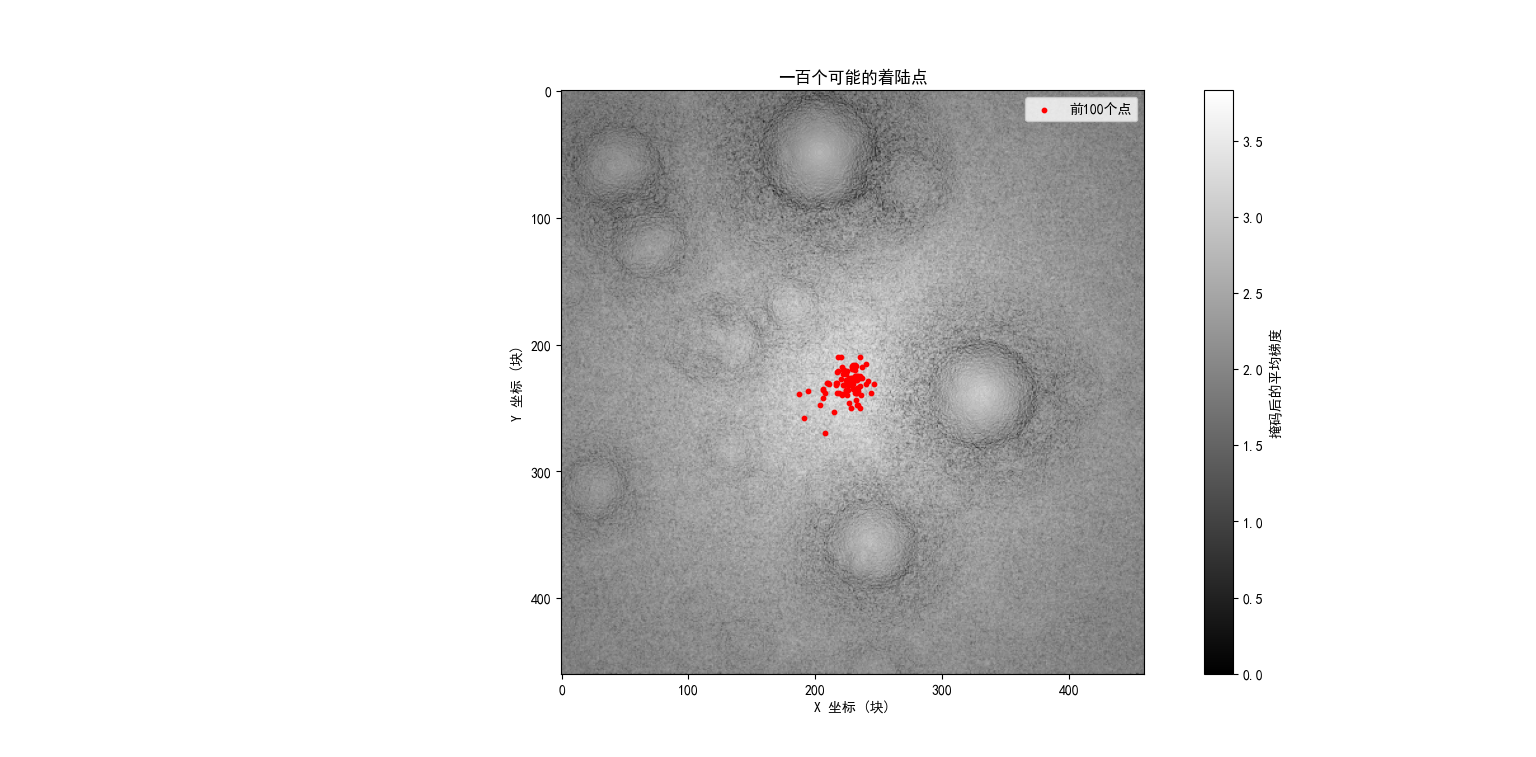
\includegraphics[width=0.9\textwidth]{"./picture/Figure_100.png"} % 图片文件名及宽度调整
        \caption{A区未去重结果图} % 图片标题
        \label{fig:example} % 图片标签
    \end{figure}

由此可见落点会随着初状态的改变而发生改变,但是落点始终集中于一定范围内,进而验证了落点选取的准确性。

\subsubsection{小结}

最终综合考虑地球重力场与基于行星历表的其他星体引力场,太阳光压与大气模型,质量瘤影响,固体潮效应和相对论效应,分别计算可能的误差情况并计算哪些误差影响最大。并综合考虑求解精度影响和发动机推力控制误差与着陆准备轨道的参数误差。最终进行对于初始值的敏感性分析,并利用蒙特卡罗方法得出仿真结果。

\section{模型评价与改进}

\subsection{模型优点}
\begin{enumerate}[(1)]
    \item 针对第二问中的问题,我们的模型能够有效地计算出每个区域的平均梯度,并通过反转灰度值和径向衰减掩码的方法,使得梯度的变化更加显著,从而更容易识别出可能的着陆点。
    \item 模型能够处理高分辨率的数字高程图数据,通过计算每个区域的平均梯度来减少计算量,同时保持较高的精度。
    \item 我们的模型通过应用径向衰减掩码,有效地减弱了远离中心区域的影响,使得可能的着陆点更加集中和明确。
    \item 模型进行了数据处理和可视化,具有较强的灵活性和可扩展性,可以方便地进行进一步的调整和改进。
\end{enumerate}

\subsection{模型缺点}
\begin{enumerate}[(1)]
    \item 问题一中的处理方法较为简单,没有考虑到更复杂的地形特征和地形数据的潜在误差。未来可以考虑引入更复杂的地形分析算法,如地形粗糙度分析等,以提高模型的精度。在计算径向衰减掩码时,使用了固定的衰减速度。实际上,不同区域的地形特征可能需要不同的衰减速度。未来可以考虑通过优化算法自动调整衰减速度,以提高模型的适应性。模型目前仅对数字高程图数据进行了处理,没有结合其他可能影响着陆点选择的因素,如地质特征。
\end{enumerate}


    \begin{thebibliography}{9} % 参考文献
		\bibitem{bib:11}[1]黄勇."嫦娥一号"探月飞行器的轨道计算研究[D].中国科学院研究生院(上海天文台),2006.
		\bibitem{bib:8}何晓群.多元统计分析.北京:中国人民大学出版社,2012.
		\bibitem{bib:9}徐维超. 相关系数研究综述[J]. 广东工业大学学报,2012,29(3):12-17.
		\bibitem{bib:10}杜劲松, 陈超, 梁青, 张毅. 月球重力异常及其计算方法[J]. 武汉大学学报 ( 信息科学版), 2012, 37(11): 1369-1373.
		\bibitem{bib:12}沈祖炜.阿波罗登月舱最终下降及着陆综述[J].航天返回与遥感,2008,29(1):5.DOI:10.3969/j.issn.1009-8518.2008.01.003.
		\bibitem{bib:13}阿波罗登月舱最终下降及着陆综述[J].沈祖炜.(北京空间机电研究所 北京 100076)

    \end{thebibliography}

    \newpage
    \section{附录}
% 第一个代码块
\begin{lstlisting}[language=Python, caption={主代码}, xleftmargin=0pt]
import matplotlib.pyplot as plt
import math


R=1737.1e3
def vector_object(v):
    return [-v[0], -v[1]]
def vector_add(v1, v2):
    return [v1[0] + v2[0], v1[1] + v2[1]]

def vector_sub(v1, v2):
    return [v1[0] - v2[0], v1[1] - v2[1]]

def vector_mul_scalar(v, s):
    return [v[0] * s, v[1] * s]

def vector_div_scalar(v, s):
    return [v[0] / s, v[1] / s]

def vector_magnitude(v):
    return math.sqrt(v[0]**2 + v[1]**2)

def vector_unit(v):
    mag = vector_magnitude(v)
    return [v[0] / mag, v[1] / mag]

def rotate_vector_left_90_degrees(v):
    """
    将二维向量右转90度
    参数:
    v: 向量 (列表形式, [x, y])
    返回:
    v_rotated: 右转90度后的向量 (列表形式, [y, -x])
    """
    x, y = v
    v_rotated = [-y, x]
    return v_rotated

def rotate_vector_right_90_degrees(v):
    """
    将二维向量右转90度
    参数:
    v: 向量 (列表形式, [x, y])
    返回:
    v_rotated: 右转90度后的向量 (列表形式, [y, -x])
    """
    x, y = v
    v_rotated = [y, -x]
    return v_rotated

def decompose_velocity(v, en):
    """
    将速度向量分解为径向速度和切向速度
    参数:
    v: 速度向量 (列表形式, [vx, vy])
    en: 径向单位向量 (列表形式, [ex, ey])
    返回:
    vr: 径向速度 (标量)
    vt: 切向速度向量 (列表形式, [vtx, vty])
    """
    # 计算径向速度 (标量)
    vr = v[0] * en[0] + v[1] * en[1]
    # 计算切向速度向量
    vt = [v[0] - vr * en[0], v[1] - vr * en[1]]
    vt = vector_magnitude(vt)
    return vr, vt

def vector_dot_product(v1, v2):
    """
    计算两个二维向量的点积

    参数:
    v1: 第一个向量 (列表形式, [x1, y1])
    v2: 第二个向量 (列表形式, [x2, y2])

    返回:
    dot_product: 点积 (标量)
    """
    return v1[0] * v2[0] + v1[1] * v2[1]

def simulate_moon_landing(m, r0, v0, dt, t_max, G=6.67430e-11, M=7.342e22, R=1737.1e3-2641):
    """
    模拟飞船在月球上的着陆过程

    参数:
    m: 飞船质量 (kg)
    r0: 初始位置向量 (列表, 米)
    v0: 初始速度向量 (列表, 米/秒)
    dt: 时间步长 (秒)
    t_max: 总模拟时间 (秒)
    G: 引力常数 (m^3 kg^-1 s^-2)
    M: 月球质量 (kg)
    R: 月球半径 (米)
    burn_time: 减速开始的时间 (秒)
    thrust_duration: 推力作用时间 (秒)
    thrust_magnitude: 推力加速度的大小 (m/s^2)
    thrust_direction: 推力方向单位向量 (列表)

    返回:
    r: 位置向量随时间变化的数组 (米)
    v: 速度向量随时间变化的数组 (米/秒)
    """
    # 初始化位置、速度和加速度
    r = r0[:]
    v = v0[:]
    positions = [r[:]]
    velocities = [v[:]]
    dms = 2.55102040
    ve = 2940
    t = 0
    while t < t_max:
        # 计算引力加速度
        r_magnitude = vector_magnitude(r)
        a_gravity = vector_mul_scalar(r, -G * M / r_magnitude**3)
        #thrust_direction = rotate_vector_90_degrees(vector_unit(r))
        v_h = vector_object(vector_unit(decompose_velocity(v, vector_unit(r))))
        thrust_direction_en = [3.74684*v_h[0], v_h[1]]
        thrust_direction_t = vector_mul_scalar(rotate_vector_right_90_degrees(vector_unit(r)), thrust_direction_en[1])
        thrust_direction_n = vector_mul_scalar(vector_unit(r), thrust_direction_en[0])
        thrust_direction = vector_unit(vector_add(thrust_direction_t,thrust_direction_n))
        thrust_magnitude = (dms*ve)/m
        # 计算推力加速度
        if (decompose_velocity(v,vector_unit(r))[0]**2+decompose_velocity(v,vector_unit(r))[1]**2)**0.5 > 57:
            a_thrust = vector_mul_scalar(thrust_direction, thrust_magnitude)
            m -= dms * dt
        else:
            print(t)
            print(decompose_velocity(v, vector_unit(r)))
            print(m, m0-m)
            print(vector_magnitude(r)-R)
            a_thrust = [0, 0]
            break
        # 总加速度
        a_total = vector_add(a_gravity, a_thrust)
        # 更新速度
        v_new = vector_add(v, vector_mul_scalar(a_total, dt))
        # 更新位置
        r_new = vector_add(r, vector_add(vector_mul_scalar(v, dt), vector_mul_scalar(a_total, 0.5 * dt**2)))
        # 更新位置、速度
        r = r_new[:]
        v = v_new[:]
        # 记录新的位置和速度
        positions.append(r[:])
        velocities.append(v[:])
        # 更新时间
        t += dt
    input(':')
    # stage 2
    dms = 1.058
    while t < t_max:
        # 计算引力加速度
        r_magnitude = vector_magnitude(r)
        a_gravity = vector_mul_scalar(r, -G * M / r_magnitude**3)
        #thrust_direction = rotate_vector_90_degrees(vector_unit(r))
        v_h = vector_object(vector_unit(decompose_velocity(v, vector_unit(r))))
        thrust_direction_en = [v_h[0], v_h[1]]
        thrust_direction_t = vector_mul_scalar(rotate_vector_right_90_degrees(vector_unit(r)), thrust_direction_en[1])
        thrust_direction_n = vector_mul_scalar(vector_unit(r), thrust_direction_en[0])
        thrust_direction = vector_unit(vector_add(thrust_direction_t,thrust_direction_n))
        thrust_magnitude = (dms*ve)/m
        # 计算推力加速度
        if decompose_velocity(v,vector_unit(r))[1] > 0.1:
            a_thrust = vector_mul_scalar(thrust_direction, thrust_magnitude)
            m -= dms * dt
        else:
            print(t)
            print(decompose_velocity(v, vector_unit(r)))
            print(m, m0-m)
            print(vector_magnitude(r)-R)
            a_thrust = [0, 0]
            break
        # 总加速度
        a_total = vector_add(a_gravity, a_thrust)
        # 更新速度
        v_new = vector_add(v, vector_mul_scalar(a_total, dt))
        # 更新位置
        r_new = vector_add(r, vector_add(vector_mul_scalar(v, dt), vector_mul_scalar(a_total, 0.5 * dt**2)))
        # 更新位置、速度
        r = r_new[:]
        v = v_new[:]
        # 记录新的位置和速度
        positions.append(r[:])
        velocities.append(v[:])
        # 更新时间
        t += dt
    input(':')
    # stage 3
    dms = 0
    while t < t_max:
        # 计算引力加速度
        r_magnitude = vector_magnitude(r)
        a_gravity = vector_mul_scalar(r, -G * M / r_magnitude ** 3)
        # 计算推力加速度
        if vector_magnitude(r) - R > 741:
            a_thrust = [0, 0]
        else:
            print(t)
            print(decompose_velocity(v, vector_unit(r)))
            print(m, m0-m)
            print(vector_magnitude(r)-R)
            break
        # 总加速度
        a_total = vector_add(a_gravity, a_thrust)
        # 更新速度
        v_new = vector_add(v, vector_mul_scalar(a_total, dt))
        # 更新位置
        r_new = vector_add(r, vector_add(vector_mul_scalar(v, dt), vector_mul_scalar(a_total, 0.5 * dt ** 2)))
        # 更新位置、速度
        r = r_new[:]
        v = v_new[:]
        # 记录新的位置和速度
        positions.append(r[:])
        velocities.append(v[:])
        # 更新时间
        t += dt
    input(':')
    # stage 4
    dms = 2.55102040
    while t < t_max:
        # 计算引力加速度
        r_magnitude = vector_magnitude(r)
        a_gravity = vector_mul_scalar(r, -G * M / r_magnitude ** 3)
        # thrust_direction = rotate_vector_90_degrees(vector_unit(r))
        thrust_direction = vector_object(vector_unit(v))
        thrust_magnitude = (dms * ve) / m
        # 计算推力加速度
        if decompose_velocity(v, vector_unit(r))[0] < -0.1:
            a_thrust = vector_mul_scalar(thrust_direction, thrust_magnitude)
            m -= dms * dt
        else:
            print(t)
            print(decompose_velocity(v, vector_unit(r)))
            print(m, m0-m)
            print(vector_magnitude(r)-R)
            a_thrust = [0, 0]
            break
        # 总加速度
        a_total = vector_add(a_gravity, a_thrust)
        # 更新速度
        v_new = vector_add(v, vector_mul_scalar(a_total, dt))
        # 更新位置
        r_new = vector_add(r, vector_add(vector_mul_scalar(v, dt), vector_mul_scalar(a_total, 0.5 * dt ** 2)))
        # 更新位置、速度
        r = r_new[:]
        v = v_new[:]
        # 记录新的位置和速度
        positions.append(r[:])
        velocities.append(v[:])
        # 更新时间
        t += dt
    input(':')
    # stage 5
    dms = 0
    while t < t_max:
        # 计算引力加速度
        r_magnitude = vector_magnitude(r)
        a_gravity = vector_mul_scalar(r, -G * M / r_magnitude ** 3)
        # 计算推力加速度
        if vector_magnitude(r) - R > 30.1:
            a_thrust = [0, 0]
        else:
            print(t)
            print(decompose_velocity(v, vector_unit(r)))
            print(m, m0-m)
            print(vector_magnitude(r)-R)
            a_thrust = [0, 0]
            break
        # 总加速度
        a_total = vector_add(a_gravity, a_thrust)
        # 更新速度
        v_new = vector_add(v, vector_mul_scalar(a_total, dt))
        # 更新位置
        r_new = vector_add(r, vector_add(vector_mul_scalar(v, dt), vector_mul_scalar(a_total, 0.5 * dt ** 2)))
        # 更新位置、速度
        r = r_new[:]
        v = v_new[:]
        # 记录新的位置和速度
        positions.append(r[:])
        velocities.append(v[:])
        # 更新时间
        t += dt
    input(':')
    # stage 6
    dms = 2.55102040
    while t < t_max:
        # 计算引力加速度
        r_magnitude = vector_magnitude(r)
        a_gravity = vector_mul_scalar(r, -G * M / r_magnitude ** 3)
        # thrust_direction = rotate_vector_90_degrees(vector_unit(r))
        thrust_direction = vector_object(vector_unit(v))
        thrust_magnitude = (dms * ve) / m
        # 计算推力加速度
        if decompose_velocity(v, vector_unit(r))[0] < 0:
            a_thrust = vector_mul_scalar(thrust_direction, thrust_magnitude)
            m -= dms * dt
        else:
            print(t)
            print(decompose_velocity(v, vector_unit(r)))
            print(m, m0-m)
            print(vector_magnitude(r)-R)
            a_thrust = [0, 0]
            break
        # 总加速度
        a_total = vector_add(a_gravity, a_thrust)
        # 更新速度
        v_new = vector_add(v, vector_mul_scalar(a_total, dt))
        # 更新位置
        r_new = vector_add(r, vector_add(vector_mul_scalar(v, dt), vector_mul_scalar(a_total, 0.5 * dt ** 2)))
        # 更新位置、速度
        r = r_new[:]
        v = v_new[:]
        # 记录新的位置和速度
        positions.append(r[:])
        velocities.append(v[:])
        # 更新时间
        t += dt
    input(':')
    # stage 7
    dms = 0
    while t < t_max:
        # 计算引力加速度
        r_magnitude = vector_magnitude(r)
        a_gravity = vector_mul_scalar(r, -G * M / r_magnitude ** 3)
        # 总加速度
        a_total = vector_add(a_gravity, a_thrust)
        # 更新速度
        v_new = vector_add(v, vector_mul_scalar(a_total, dt))
        # 更新位置
        r_new = vector_add(r, vector_add(vector_mul_scalar(v, dt), vector_mul_scalar(a_total, 0.5 * dt ** 2)))
        # 检查是否到达月球表面
        if vector_magnitude(r) <= R:
            print(decompose_velocity(v, vector_unit(r)))
            print(m, m0 - m)
            print(vector_magnitude(r) - R)
            print(f"Landing successful at time {t} seconds.")
            print(vector_magnitude(v))
            break
        # 更新位置、速度
        r = r_new[:]
        v = v_new[:]
        # 记录新的位置和速度
        positions.append(r[:])
        velocities.append(v[:])
        # 更新时间
        t += dt
    input(':')
    return positions, velocities

# 参数设置
m0 = 2400  # 飞船质量 (kg)
r0 = [0, R + 15000]  # 初始位置 (米), 轨道高度为100km
v0 = [1692, 0]  # 初始速度 (米/秒), 在近月点的速度
dt = 0.001  # 时间步长 (秒)
t_max = 1000  # 总模拟时间 (秒), 模拟1小时
# 计算轨迹
positions, velocities = simulate_moon_landing(m0, r0, v0, dt, t_max)

# 可视化轨迹
fig, ax = plt.subplots(figsize=(10, 10))
positions_x = [pos[0] for pos in positions]
positions_y = [pos[1] for pos in positions]
ax.plot(positions_x, positions_y, label='Spacecraft Trajectory')

# 绘制月球
moon = plt.Circle((0, 0), 1737.4e3, color='gray', alpha=0.5)
ax.add_artist(moon)

# 标注月球中心
ax.plot(0, 0, 'ro', label='Moon Center')

# 设置图形属性
ax.set_xlabel('x (m)')
ax.set_ylabel('y (m)')
ax.set_title('Trajectory of Spacecraft Landing on Moon')
ax.legend()
ax.grid(True)
ax.set_aspect('equal')
ax.set_xlim([-2e6, 2e6])
ax.set_ylim([-2e6, 2e6])

plt.show()

\end{lstlisting}

% 第二个代码块
\begin{lstlisting}[language=Python, caption={寻找最优着陆点代码}, xleftmargin=0pt]
import numpy as np
import matplotlib.pyplot as plt
import rasterio
from sklearn.cluster import KMeans

# 读取高程图数据
tif_file = '附件3 距2400m处的数字高程图.tif'
with rasterio.open(tif_file) as src:
    elevation_data = src.read(1)  # 读取第一波段数据

# 计算梯度
gradient_y, gradient_x = np.gradient(elevation_data)

# 获取数据的形状
height, width = elevation_data.shape

# 定义块大小
block_size = 5

# 创建一个新的数组来存储每个 5x5 区域的平均梯度
avg_gradients = np.zeros((height // block_size, width // block_size))

# 计算每个 5x5 区域的平均梯度
for i in range(0, height, block_size):
    for j in range(0, width, block_size):
        # 获取当前区域
        block_grad_x = gradient_x[i:i + block_size, j:j + block_size]
        block_grad_y = gradient_y[i:i + block_size, j:j + block_size]

        # 计算当前区域的平均梯度大小
        block_grad_magnitude = np.sqrt(block_grad_x ** 2 + block_grad_y ** 2)
        avg_grad_magnitude = np.mean(block_grad_magnitude)

        # 存储结果
        avg_gradients[i // block_size, j // block_size] = avg_grad_magnitude

# 反转灰度值
avg_gradients_inverted = np.max(avg_gradients) - avg_gradients

# 创建径向衰减掩码,调整衰减速度
center_x, center_y = width / 2, height / 2
y, x = np.ogrid[:height, :width]
distance_from_center = np.sqrt((x - center_x)**2 + (y - center_y)**2)
decay_speed = 0.0005  # 调整衰减速度
mask = 1 / (decay_speed * distance_from_center + 1)  # 防止除以零

# 缩放掩码到 5x5 块的大小
mask_small = mask[::block_size, ::block_size]

# 应用掩码到反转后的平均梯度
avg_gradients_masked = avg_gradients_inverted * mask_small[:avg_gradients.shape[0], :avg_gradients.shape[1]]

# 获取结果中值最大的100个像素点
flattened_indices = np.argsort(avg_gradients_masked, axis=None)[-5:][::-1]
flattened_indices.sort()
print(flattened_indices)
coords = np.unravel_index(flattened_indices, avg_gradients_masked.shape)
values = avg_gradients_masked[coords]

# 聚类
points = np.column_stack((coords[1] * block_size + block_size / 2, coords[0] * block_size + block_size / 2))
print(points)
kmeans = KMeans(n_clusters=5, random_state=0).fit(points)
cluster_centers = kmeans.cluster_centers_

# 计算聚类中心与图片中心的距离
distances = np.sqrt((cluster_centers[:, 0] - center_x)**2 + (cluster_centers[:, 1] - center_y)**2)

# 显示反转并应用掩码后的梯度灰度图,并标记最大的100个像素点和聚类中心
plt.figure(figsize=(10, 8))
plt.imshow(avg_gradients_masked, cmap='gray', extent=(0, width, height, 0))
plt.colorbar(label='Inverted Average Gradient Magnitude with Radial Decay Mask')
plt.title('Inverted Average Gradient Map (5x5 blocks) with Radial Decay Mask')
plt.xlabel('X Coordinate')
plt.ylabel('Y Coordinate')
# 标记最大的100个像素点
plt.scatter(points[:, 0], points[:, 1], color='red', s=10, label='Top 100 Points')
# 标记聚类中心
plt.scatter(cluster_centers[:, 0], cluster_centers[:, 1], color='blue', s=50, marker='x', label='Cluster Centers')
plt.legend()
plt.show()

# 输出聚类中心与图片中心的距离
print(distances)

\end{lstlisting}
\end{document}